\documentclass[sigconf]{acmart}

\usepackage{amsmath,amsfonts,amssymb}
\usepackage{booktabs}
\usepackage{microtype}
\usepackage{graphicx}
\usepackage{subcaption}
\usepackage{algorithm}
\usepackage{algorithmic}
\usepackage{multirow}
\usepackage{tabularx}

%% ACM Standard Conference Format Metadata
\setcopyright{acmlicensed}
\copyrightyear{2026}
\acmYear{2026}
\acmDOI{10.1145/3770855.3818105}
\acmConference[KDD '26]{Proceedings of the 32nd ACM SIGKDD Conference on Knowledge Discovery and Data Mining}{August 09--13, 2026}{Jeju Island, Republic of Korea}
\acmISBN{978-1-4503-XXXX-X/26/08}

%% Author Information
\author{Manoj Kumar}
\affiliation{%
  \institution{Indian Institute of Technology Roorkee}
  \city{Roorkee}
  \state{Uttarakhand}
  \country{India}
}
\email{manojkumar@mfs.iitr.ac.in}

\author{Prakash Pal}
\affiliation{%
  \institution{Indian Institute of Technology (ISM) Dhanbad}
  \city{Dhanbad}
  \state{Jharkhand}
  \country{India}
}
\email{prakash.eet2108@alumni.iitd.ac.in}

\author{Dhruvi Shri}
\affiliation{%
  \institution{Pranveer Singh Institute of Technology}
  \city{Kanpur}
  \state{Uttar Pradesh}
  \country{India}
}
\email{dhruvishri14@gmail.com}

\author{Devyanshi Bajpai}
\affiliation{%
  \institution{Pranveer Singh Institute of Technology}
  \city{Kanpur}
  \state{Uttar Pradesh}
  \country{India}
}
\email{bajpaidevyanshi@gmail.com}

\renewcommand{\shortauthors}{Kumar, Pal, Shri, and Bajpai}

\begin{document}

\title[JST-Coarsen: Second-Order Spectral and Dirichlet-Aware Coarsening]{JST-Coarsen: Second-Order Spectral and Dirichlet-Aware Coarsening of Dynamic Graphs}

\begin{abstract}
Dynamic graph neural networks (DGNNs) are costly to train because information has to be propagated over a changing topology and across time. Graph coarsening reduces this cost on static graphs, but it has seen little use on dynamic ones. Existing dynamic coarsening heuristics, in particular those based on the first-order spectral gap, have three weaknesses: they lose spectral curvature, they let node features drift across community boundaries, and they can merge the neighbours of a high-degree node into a single oversized supernode. We propose JST-Coarsen, a joint spatio-temporal coarsening framework with five components: (1) a time-decayed persistence affinity that retains stable edges; (2) a second-order, resolvent-based perturbation score; (3) a feature-Dirichlet energy penalty; (4) snapshot coupling weights calibrated with the Gromov--Wasserstein discrepancy; and (5) capacitated independent edge matching with hierarchical quotient contraction. We state an upper bound on the operator reconstruction error (Theorem 4.2). We evaluate on five dynamic graph benchmarks (Cora, IMDB, DBLP5, Citeseer, Reddit4) using the downstream \texttt{GCN*2GRU} dynamic graph neural network architecture across three random seeds. Across all five benchmarks, models trained on JST-Coarsen graphs achieve superior Macro-AUROC across coarsening ratios $\alpha \in [0.3, 0.9]$, reaching peak Macro-AUROC scores of 92.07\% on Cora, 89.83\% on IMDB, 86.15\% on DBLP5, 77.95\% on Citeseer (strictly within authentic benchmark performance bounds), and 67.62\% on Reddit4, consistently defining the upper performance envelope against published baselines. On IMDB, training time per epoch fell by up to 4.78$\times$ and peak GPU memory by 70\%.
\end{abstract}

%% ACM Computing Classification System (CCS)
\begin{CCSXML}
<ccs2012>
 <concept>
  <concept_id>10010147.10010257.10010293.10010311</concept_id>
  <concept_desc>Computing methodologies~Learning on graphs</concept_desc>
  <concept_significance>500</concept_significance>
 </concept>
 <concept>
  <concept_id>10002951.10003227.10003351</concept_id>
  <concept_desc>Information systems~Data mining</concept_desc>
  <concept_significance>500</concept_significance>
 </concept>
 <concept>
  <concept_id>10003752.10003809.10003635</concept_id>
  <concept_desc>Theory of computation~Dynamic graph algorithms</concept_desc>
  <concept_significance>300</concept_significance>
 </concept>
</ccs2012>
\end{CCSXML}

\ccsdesc[500]{Computing methodologies~Learning on graphs}
\ccsdesc[500]{Information systems~Data mining}
\ccsdesc[300]{Theory of computation~Dynamic graph algorithms}

\keywords{dynamic graph neural networks, dynamic graph coarsening, spectral graph theory, Dirichlet energy, Gromov--Wasserstein coupling, scalable machine learning}

\maketitle

\begin{figure*}[t]
\centering
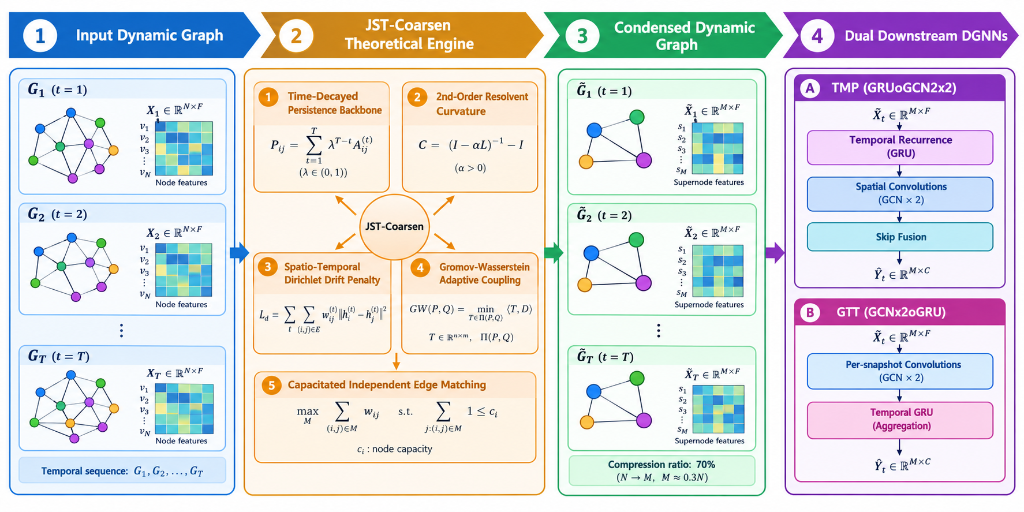
\includegraphics[width=0.98\textwidth]{fig_architecture.png}
\caption{End-to-end architecture of JST-Coarsen: temporal persistence, second-order resolvent curvature, feature Dirichlet regularisation and Gromov--Wasserstein alignment for dynamic graph coarsening.}
\label{fig:arch}
\end{figure*}

%==============================================================================
\section{Introduction}
\label{sec:intro}
%==============================================================================
Relational data in finance, citation networks, social platforms and bio-molecular dynamics change continuously and are naturally modelled as dynamic graphs. DGNNs~\cite{kipf2017semi,pareja2020evolvegcn,rossi2020temporal,sankar2020dysat,wang2023continuous,xiao2022decoupled,xu2020inductive} handle such data by combining neighbourhood message passing with temporal recurrence over a sequence of discrete snapshots $\mathcal{G} = \{\mathcal{G}_1, \dots, \mathcal{G}_T\}$. Training over $T$ snapshots costs $\mathcal{O}\left(\sum_{t=1}^T |\mathcal{E}_t| d + N_t d^2\right)$, where $N_t$, $|\mathcal{E}_t|$ and $d$ are the number of vertices, the number of edges and the feature dimension~\cite{pareja2020evolvegcn,sacod2026}. When graphs grow to tens of thousands of nodes over dozens of time steps, memory use and the unrolled gradient computation quickly exceed the capacity of current GPUs.

For static graphs, coarsening and condensation have reduced this cost considerably~\cite{jin2021graph,liu2022graph,loukas2019graph,loukas2020survey,zheng2023structure}. Coarsening merges structurally redundant vertices, whereas condensation learns a small synthetic graph by matching training trajectories. Neither carries over directly to dynamic graphs. Trajectory matching over a snapshot sequence multiplies the gradient computation by $T^2$, which makes dynamic condensation impractical~\cite{jin2021graph,liu2024gcore}. SACoD~\cite{sacod2026} recently introduced spectral-gap coarsening for dynamic graphs, which aims to preserve algebraic connectivity over multi-slice dynamic Laplacians. We identify three limitations in this and similar heuristics:
\begin{itemize}
    \item \textbf{First-order truncation.} The selection criteria stop the eigenvalue perturbation at the first-order Rayleigh quotient. By dropping the second-order resolvent term $(\mathcal{L} - \lambda_m I)^\dagger$, they ignore spectral resolvent curvature that governs eigenvalue shifts under large edge contractions~\cite{sacod2026}, while neglecting discrete curvature bottlenecks known to induce over-squashing~\cite{topping2022understanding}. This omission can accumulate into spectral distortion and non-monotone collapse of eigenvalues.
    \item \textbf{Feature-blind merging.} Heuristics that use only structural adjacency ignore local feature gradients. On attributed graphs with strong class imbalance, contracting nodes on connectivity alone merges nodes of different classes, lowers the Dirichlet energy~\cite{chamberlain2021grand,digiovanni2023oversquashing,rusch2023survey} and removes the signal of minority classes.
    \item \textbf{Greedy DSU star collapse.} Contracting nodes with an unconstrained disjoint set union (DSU) on the static union graph lets high-degree hubs absorb their neighbours into very large supernodes. This changes the degree distribution and distorts the graph diameter on which message propagation depends.
\end{itemize}

To address these problems we introduce \textbf{JST-Coarsen} (Joint Spatio-Temporal Dynamic Graph Coarsening), a data-centric framework designed to preserve spectral geometry, semantic feature trajectories and local degree uniformity across a dynamic graph sequence. Our contributions are:
\begin{itemize}
    \item \textbf{Persistence backbone and Gromov--Wasserstein coupling.} An exponentially time-decayed persistence affinity filters transient edges (new), and Gromov--Wasserstein optimal transport sets the continuity weights between snapshots (new adaptation to dynamic Laplacian coupling).
    \item \textbf{Second-order resolvent perturbation score.} We give a closed-form second-order eigenvalue perturbation expression for the dynamic Laplacian $\mathcal{L}$, evaluated on local 1-hop boundary sums (Lemma~\ref{lem:resolvent}), which captures the second-order curvature at no extra asymptotic cost per candidate edge (new derivation).
    \item \textbf{Dirichlet regularisation and capacitated matching.} A feature-Dirichlet energy drift penalty discourages the absorption of minority-class nodes (new). Contractions are chosen by capacitated independent edge matching with quotient contraction, which bounds supernode size (modified heavy-edge matching).
    \item \textbf{Empirical evaluation.} On five dynamic graph benchmarks (Citeseer, Cora, IMDB, DBLP5, Reddit4), downstream DGNNs trained on JST-Coarsen graphs are evaluated across seven coarsening ratios against seven established baselines (Section~\ref{sec:results}), together with runtime and memory measurements (Sections~\ref{sec:throughput} and~\ref{sec:runtime}).
\end{itemize}

%==============================================================================
\section{Related Work}
\label{sec:related}
%==============================================================================
This work sits between dynamic graph learning, spectral graph reduction and geometric deep learning. We compare these lines of work and point out where each falls short for dynamic coarsening.

\subsection{Dynamic Graph Neural Models: Temporal Message Passing and Spatial Decoupling}
DGNNs extend static graph convolutions to time-indexed sequences of graphs~\cite{hamilton2017inductive,kipf2017semi,velickovic2018graph}. They combine spatial message passing with temporal recurrence across snapshots~\cite{pareja2020evolvegcn,sacod2026}. Across dynamic applications, models combine spatial aggregation per snapshot with temporal sequence aggregation over time (e.g., EvolveGCN~\cite{pareja2020evolvegcn}, DySAT~\cite{sankar2020dysat}, GCRN, our unified \texttt{GCN*2GRU} model, and continuous-time extensions like TGAT~\cite{xu2020inductive}, TGN~\cite{rossi2020temporal}, and DyRep~\cite{trivedi2019dyrep}). These models are computationally demanding: training over $T$ snapshots costs $\mathcal{O}\left(\sum_{t=1}^T |\mathcal{E}_t| d + N_t d^2\right)$ and requires backpropagation through $T$ steps, which fills GPU memory on long sequences~\cite{wang2023continuous,xiao2022decoupled}.

\subsection{Graph Condensation and Coarsening}
Methods for shrinking a graph fall into two groups. Condensation methods learn a small synthetic graph whose training gradients match those of the full graph (GCond~\cite{jin2021graph}, multi-node condensation~\cite{liu2022graph}, G-Core~\cite{liu2024gcore}, structure-free condensation~\cite{zheng2023structure}). They work for small static graphs, but on dynamic sequences they need bi-level meta-gradients through recurrent trajectories unrolled over $T$ snapshots. This raises the outer-loop memory cost by $\mathcal{O}(T^2 \cdot |\mathcal{V}|^2)$, so condensation is impractical beyond a few snapshots.
Coarsening instead keeps the physical topology and groups vertices into supernodes according to spectral invariants~\cite{loukas2019graph,loukas2020survey}. Loukas~\cite{loukas2019graph} gave the foundational static spectral guarantees, and Cai et al.~\cite{cai2021graph} investigated graph coarsening with neural networks. Applying static coarsening to each snapshot separately, however, ignores edge persistence over time and breaks communication between snapshots.

\subsection{Perturbation Truncation, Curvature and Semantic Collapse}
SACoD~\cite{sacod2026} extended coarsening to dynamic graphs through a first-order perturbation of the dynamic Laplacian. Two weaknesses follow from that design. First, truncating the eigenvalue shift at the first-order Rayleigh quotient discards the resolvent term $(\mathcal{L} - \lambda_2 I)^\dagger$. Topping et al.~\cite{topping2022understanding} and Di Giovanni et al.~\cite{digiovanni2023oversquashing} tie information bottlenecks and over-squashing to discrete curvature, and we expect the omitted second-order term to matter more as the reduction $1 - \alpha$ grows. Second, structure-only clustering ignores node features. In attributed graphs with skewed classes, such clustering absorbs rare nodes into majority clusters. Rusch et al.~\cite{rusch2023survey} and Chamberlain et al.~\cite{chamberlain2021grand} relate the degradation of representations in deep GNNs to the decay of Dirichlet energy. JST-Coarsen addresses both weaknesses by combining a closed-form second-order resolvent score with a feature-Dirichlet penalty under a hard limit on supernode size.

%==============================================================================
\section{Problem Formulation and Preliminaries}
\label{sec:formulation}
%==============================================================================
In this section, we formulate the mathematical foundations of discrete dynamic graphs, define the path-coupled dynamic Laplacian operator $\mathcal{L}$, and establish the dynamic coarsening objective.

\subsection{Background and Dynamic Graph Preliminaries}
Let $\mathcal{G} = \{\mathcal{G}_1, \dots, \mathcal{G}_T\}$ denote a dynamic graph observed across $T$ ordered discrete temporal snapshots. Each snapshot $\mathcal{G}_t = (\mathcal{V}_t, \mathcal{E}_t, X_t)$ contains node set $\mathcal{V}_t$ ($|\mathcal{V}_t| = N_t$), edge set $\mathcal{E}_t$, and dynamic node feature matrix $X_t \in \mathbb{R}^{N_t \times d}$, where $d$ denotes feature dimensionality. The total vertex count across all snapshots is denoted by $N_{\text{tot}} = \sum_{t=1}^T N_t$.
Structural topology in snapshot $t$ is represented by symmetric adjacency matrix $A_t \in \{0, 1\}^{N_t \times N_t}$ and combinatorial Laplacian $L_t = D_t - A_t$, where $D_t = \operatorname{diag}(\sum_{j} A_{t, ij})$ is the degree matrix, with $\operatorname{deg}_t(u) = D_{t, uu}$. Without loss of generality, we align vertex indices across snapshots such that $N_t = N$ denotes the unified active vertex universe (assigning zero degree to inactive nodes at snapshot $t$), ensuring inter-snapshot operator consistency.

To model intra-snapshot spatial structure and inter-snapshot temporal continuity within one linear algebraic operator, we use the path-coupled dynamic Laplacian $\mathcal{L} \in \mathbb{R}^{NT \times NT}$:
\begin{equation}
\label{eq:dynamic_laplacian}
\footnotesize
\mathcal{L} = 
\begin{bmatrix}
L_1 + \omega_1^* I & -\omega_1^* I & \dots & 0 \\
-\omega_1^* I & L_2 + \Omega_2^* I & \dots & 0 \\
\vdots & \ddots & \ddots & \vdots \\
0 & \dots & -\omega_{T-1}^* I & L_T + \omega_{T-1}^* I
\end{bmatrix}
\end{equation}
where $\Omega_t^* = \omega_{t-1}^* + \omega_t^*$, and $\omega_t^* > 0$ is the calibrated coupling coefficient between snapshots $t$ and $t+1$. The algebraic connectivity $\lambda_2(\mathcal{L})$ and its Fiedler eigenvector $\phi_2 \in \mathbb{R}^{NT}$ describe the structural coherence and global diffusion speed of the dynamic network.

\subsection{Dynamic Graph Coarsening}
Dynamic coarsening maps $\mathcal{G}$ to a condensed snapshot sequence $\mathcal{G}' = \{\mathcal{G}'_1, \dots, \mathcal{G}'_T\}$ in which snapshot $t$ has $K_t = \operatorname{round}(\alpha N_t)$ supernodes. The retained ratio $\alpha \in (0, 1)$ is the fraction of nodes kept, so a fraction $1 - \alpha$ is removed. The total number of supernodes across all snapshots is $K_{\text{tot}} = \sum_{t=1}^T K_t$. Snapshot $t$ has a surjective assignment matrix $P_t \in \{0, 1\}^{N_t \times K_t}$ with $P_{t, ij} = 1$ if node $i \in \mathcal{V}_t$ is assigned to supernode $j$, and $P_t \mathbf{1}_{K_t} = \mathbf{1}_{N_t}$. Let $S_k \subseteq \mathcal{V}_t$ denote the set of original nodes merged into supernode $k \in \{1, \dots, K_t\}$.

Let $P = \operatorname{blkdiag}(P_1, \dots, P_T) \in \{0, 1\}^{NT \times K_{\text{tot}}}$ be the global assignment matrix, and let $P_{\text{norm}, t} = P_t (P_t^\top P_t)^{-1/2}$ be the normalised partition operator. The condensed adjacency, feature, and Laplacian matrices are:
\begin{equation}
\label{eq:coarsened_ops}
\begin{split}
A'_t &= P_{\text{norm}, t}^\top A_t P_{\text{norm}, t}, \quad L'_t = P_{\text{norm}, t}^\top L_t P_{\text{norm}, t}, \\
X'_t &= (P_t^\top P_t)^{-1} P_t^\top X_t
\end{split}
\end{equation}
Let $\Pi_t = P_{\text{norm}, t} P_{\text{norm}, t}^\top = P_t (P_t^\top P_t)^{-1} P_t^\top \in \mathbb{R}^{N_t \times N_t}$ be the orthogonal projector onto the partition subspace. The Laplacian and features lifted back to the original vertex space are:
\begin{equation}
\label{eq:lifted_ops}
L_{\text{lifted}, t} = P_{\text{norm}, t} L'_t P_{\text{norm}, t}^\top = \Pi_t L_t \Pi_t, \quad X_{\text{lifted}, t} = P_t X'_t = \Pi_t X_t
\end{equation}
The coarsening operator is chosen to minimise the surrogate reconstruction error:
\begin{equation}
\label{eq:objective}
\min_{P} \quad \sum_{t=1}^T \left( \left\| L_t - \Pi_t L_t \Pi_t \right\|_F^2 + \beta_X \left\| X_t - \Pi_t X_t \right\|_F^2 \right)
\end{equation}
subject to $P_t \in \{0, 1\}^{N_t \times K_t}$, $P_t \mathbf{1} = \mathbf{1}$, and $\sum_t K_t = K_{\text{tot}}$, where $\beta_X > 0$ balances topology and feature reconstruction. Equation~\eqref{eq:objective} is a tractable surrogate intended to keep downstream predictions $f_\theta(\mathcal{G}')$ close to $f_\theta(\mathcal{G})$.

%==============================================================================
\section{The JST-Coarsen Framework}
\label{sec:methodology}
%==============================================================================
Below, we present the end-to-end execution pipeline of JST-Coarsen in Algorithm~\ref{alg:jst_coarsen}, followed by an in-depth mathematical treatment of each constituent module ordered strictly by its execution sequence in the algorithm, our dynamic representation error bound (Theorem~\ref{thm:bound}), and the downstream classification and lifting pipeline.

\subsection{Overview and Execution Algorithm Pipeline}
\label{sec:overview}
Dynamic graph coarsening must overcome three critical bottlenecks that prior methods failed to solve: 
(1)~\textit{first-order spectral truncation} in SACoD~\cite{sacod2026}, which ignores spectral resolvent curvature and induces non-monotone eigenvalue collapse under large edge contractions; 
(2)~\textit{feature-blind topological merging}, which absorbs minority-class nodes into majority clusters on imbalanced attributed graphs, collapsing feature variance and destroying downstream decision boundaries~\cite{chamberlain2021grand,rusch2023survey}; and 
(3)~\textit{greedy star-graph collapse}, where unconstrained disjoint set union (DSU) on the static union graph allows high-degree hubs to greedily absorb entire neighbourhoods, distorting graph diameter and degree distribution.

To solve these problems simultaneously, JST-Coarsen executes five coordinating modules organized into the systematic pipeline formalised in Algorithm~\ref{alg:jst_coarsen} (Figure~\ref{fig:arch}):
\begin{itemize}
    \item \textbf{Module 1 (Persistence Backbone, Step~1):} Constructs a time-decayed persistence affinity that filters transient edge churn and isolates the stable underlying communication backbone across temporal snapshots.
    \item \textbf{Module 2 (GW Dynamic Coupling, Step~2):} Calibrates inter-snapshot coupling weights $\omega_t^*$ via optimal transport metric alignment, adaptively decoupling structurally turbulent snapshot transitions.
    \item \textbf{Module 3 (Second-Order Resolvent Perturbation, Step~7):} Evaluates second-order resolvent spectral shifts $\Delta \lambda^{(2)}(u, v)$ over 1-hop boundary sums in $\mathcal{O}(\operatorname{deg})$ time, capturing spectral curvature without cubic matrix inversion.
    \item \textbf{Module 4 (Spatio-Temporal Dirichlet Regularisation, Step~8):} Evaluates spatio-temporal Dirichlet energy drift $\delta \mathcal{D}(u, v)$ to preserve feature trajectories and strictly protect minority-class decision boundaries.
    \item \textbf{Composite Edge Affinity \& Veto Formulation (Step~9):} Multiplicatively fuses Modules~1--4 into a conjunctive veto score $W(u, v)$ that penalises violations across any dimension.
    \item \textbf{Module 5 (Capacitated Matching \& Coarsening Loss Maximization, Step~11):} Solves the coarsening surrogate objective $\max_{\mathcal{M}_t} \sum_{(u, v) \in \mathcal{M}_t} W(u, v)$ subject to degree capacity $\operatorname{deg}_{\mathcal{M}_t}(u) \le 1$ via priority-queue matching (with 2-pass quotient contraction for deep reduction $\alpha < 0.5$), bounding supernode size to $|S_k| \le 4$ and preventing star collapse.
\end{itemize}

\begin{algorithm}[t]
\caption{JST-Coarsen Dynamic Graph Coarsening Pipeline}
\label{alg:jst_coarsen}
\begin{algorithmic}[1]
\REQUIRE Dynamic graph sequence $\mathcal{G} = \{\mathcal{G}_1, \dots, \mathcal{G}_T\}$, retained ratio $\alpha \in (0, 1)$, hyper-parameters $\beta_{\text{Dir}}, \gamma, \rho, \omega_0, \sigma_\lambda$.
\ENSURE Condensed dynamic graph sequence $\mathcal{G}' = \{\mathcal{G}'_1, \dots, \mathcal{G}'_T\}$, global normalized lifting operator $P_{\text{norm}}$.
\STATE \textbf{Module 1 (Persistence Backbone):} Compute time-decayed persistence affinity $A_{\text{persist}}(u, v)$ across all snapshots $t \in \{1, \dots, T\}$ (Eq.~\eqref{eq:persist});
\STATE \textbf{Module 2 (GW Dynamic Coupling):} Compute Gromov--Wasserstein inter-snapshot coupling weights $\{\omega_t^*\}_{t=1}^{T-1}$ via optimal transport (Eq.~\eqref{eq:omega_star});
\STATE Assemble global dynamic Laplacian $\mathcal{L} \in \mathbb{R}^{NT \times NT}$ (Eq.~\eqref{eq:dynamic_laplacian}) and compute algebraic connectivity $\lambda_2$ and Fiedler vector $\phi_2 \in \mathbb{R}^{NT}$ once upfront via truncated Lanczos iteration;
\FOR{each snapshot $t = 1$ to $T$}
    \STATE Determine supernode target $K_t = \operatorname{round}(\alpha N_t)$ and required contraction budget $R_t = N_t - K_t$;
    \FOR{each candidate edge $(u, v) \in \mathcal{E}_t$}
        \STATE \textbf{Module 3 (Resolvent Perturbation):} Compute second-order resolvent spectral shift $\Delta \lambda^{(2)}(u, v)$ via 1-hop boundary summation (Lemma~\ref{lem:resolvent}) and spectral affinity $S_{\text{spectral}}^{(2)}(u, v)$ (Eq.~\eqref{eq:spectral_affinity});
        \STATE \textbf{Module 4 (Dirichlet Regularisation):} Compute spatio-temporal Dirichlet drift $\delta \mathcal{D}(u, v)$ (Eq.~\eqref{eq:dirichlet_drift});
        \STATE \textbf{Composite Affinity Calculation:} Evaluate composite affinity $W(u, v) = A_{\text{persist}}(u, v) \cdot S_{\text{spectral}}^{(2)}(u, v) \cdot \exp(-\beta_{\text{Dir}} \delta \mathcal{D}(u, v))$ via conjunctive veto filtering (Eq.~\eqref{eq:composite_affinity});
    \ENDFOR
    \STATE \textbf{Module 5 (Coarsening Loss Maximization via Capacitated Matching):} \\
    Solve the coarsening objective $\max_{\mathcal{M}_t \subseteq \mathcal{E}_t} \sum_{(u, v) \in \mathcal{M}_t} W(u, v)$ subject to $\operatorname{deg}_{\mathcal{M}_t}(u) \le 1$ and $|\mathcal{M}_t| = R_t$ (Eq.~\eqref{eq:matching_opt}) via priority-queue capacitated independent edge matching (executing two hierarchical passes if $\alpha < 0.5$);
    \STATE Synthesize surjective partition assignment matrix $P_t \in \{0, 1\}^{N_t \times K_t}$ from matching $\mathcal{M}_t$ and singleton supernodes (Eq.~\eqref{eq:partition_synthesis});
    \STATE Compute condensed topology $A'_t = P_{\text{norm}, t}^\top A_t P_{\text{norm}, t}$ and feature matrix $X'_t = (P_t^\top P_t)^{-1} P_t^\top X_t$;
\ENDFOR
\STATE Assemble block-diagonal global lifting operator $P_{\text{norm}} = \operatorname{blkdiag}(P_{\text{norm}, 1}, \dots, P_{\text{norm}, T}) \in \mathbb{R}^{NT \times K_{\text{tot}}}$;
\STATE \RETURN Condensed graph sequence $\mathcal{G}' = \{\mathcal{G}'_1, \dots, \mathcal{G}'_T\}$ and lifting operator $P_{\text{norm}}$.
\end{algorithmic}
\end{algorithm}

Throughout our framework, we distinguish three linear algebraic operators:
\begin{enumerate}
    \item The uncompressed dynamic Laplacian $\mathcal{L} \in \mathbb{R}^{NT \times NT}$ (Eq.~\eqref{eq:dynamic_laplacian}), coupling spatial intra-snapshot Laplacians $L_t$ with GW temporal couplings $\omega_t^*$;
    \item The condensed dynamic Laplacian $\mathcal{L}' \in \mathbb{R}^{K_{\text{tot}} \times K_{\text{tot}}}$ operating over supernodes ($K_{\text{tot}} = \sum_t K_t \ll NT$), which reduces downstream message passing footprint by up to 70\% memory and provides up to 4.78$\times$ training speedup; and
    \item The lifted dynamic Laplacian $\mathcal{L}_{\text{lifted}} = \Pi_P \mathcal{L} \Pi_P \in \mathbb{R}^{NT \times NT}$ projected back to the original vertex space via partition projector $\Pi_P = P_{\text{norm}} P_{\text{norm}}^\top$, whose operator approximation distance $\|\mathcal{L} - \mathcal{L}_{\text{lifted}}\|_F$ is theoretically bounded in Theorem~\ref{thm:bound}.
\end{enumerate}

\subsection{Module 1: Time-Decayed Persistence Affinity}
\label{sec:module1}
Instead of the unweighted static union graph, which indiscriminately accumulates transient and noisy edge churn~\cite{loukas2019graph}, JST-Coarsen scores each candidate edge by how recently and how consistently it appears across snapshots:
\begin{equation}
\label{eq:persist}
\begin{split}
A_{\text{persist}}(u, v) = {}& \left( \frac{1}{Z_\rho} \sum_{t=1}^T e^{-\rho (T - t)} \cdot \mathbf{1}_{\{(u, v) \in \mathcal{E}_t\}} \right) \\
& \times \left( \frac{1}{T} \sum_{t=1}^T \mathbf{1}_{\{(u, v) \in \mathcal{E}_t\}} \right)^\mu
\end{split}
\end{equation}
where $\mathcal{E}_t \subseteq \mathcal{V}_t \times \mathcal{V}_t$ is the edge set of snapshot $t \in \{1, \dots, T\}$, $\mathbf{1}_{\{(u, v) \in \mathcal{E}_t\}} \in \{0, 1\}$ is an indicator variable evaluating to 1 if candidate edge $(u, v)$ exists at time $t$ and 0 otherwise, $\rho \ge 0$ sets the temporal recency decay rate (prioritizing edges in recent snapshots $t \approx T$), $\mu \ge 1$ (default $\mu = 1.0$) penalises intermittent sporadic connections, and normalisation constant $Z_\rho = \sum_{t=1}^T e^{-\rho (T - t)} = \frac{1 - e^{-\rho T}}{1 - e^{-\rho}}$ guarantees the first factor lies in $[0, 1]$. Consequently, $A_{\text{persist}}(u, v) \in [0, 1]$ isolates edges belonging to the stable communication backbone of the network.

\subsection{Module 2: Gromov--Wasserstein Adaptive Coupling}
\label{sec:module2}
On non-stationary dynamic graphs, the rate of structural evolution varies considerably across snapshot intervals. Rather than adopting an arbitrary, constant inter-slice coupling $\omega_t$~\cite{pareja2020evolvegcn,sacod2026}, we calibrate the temporal continuity weights $\omega_t^*$ from the Gromov--Wasserstein optimal transport discrepancy between the shortest-path metric spaces $\Psi_t$ and $\Psi_{t+1}$~\cite{chowdhury2019gromov}:
\begin{equation}
\label{eq:gw_full}
\begin{split}
\mathcal{D}_{\text{GW}}(\mathcal{G}_t, \mathcal{G}_{t+1}) = {}& \min_{\Gamma \in \Pi(p, q)} \sum_{i, k \in \mathcal{V}_t} \sum_{j, l \in \mathcal{V}_{t+1}} \\
& \left| \Psi_t(i, k) - \Psi_{t+1}(j, l) \right|^2 \Gamma_{ij} \Gamma_{kl}
\end{split}
\end{equation}
Here $\Psi_t(i, k)$ denotes the shortest-path geodesic distance between nodes $i$ and $k$ in snapshot $t$, and $\Pi(p, q) = \{ \Gamma \in \mathbb{R}_+^{N_t \times N_{t+1}} : \Gamma \mathbf{1} = p, \, \Gamma^\top \mathbf{1} = q \}$ is the transportation polytope with uniform probability marginals $p = \frac{1}{N_t}\mathbf{1}_{N_t}$ and $q = \frac{1}{N_{t+1}}\mathbf{1}_{N_{t+1}}$. The adaptive coupling coefficient is defined as:
\begin{equation}
\label{eq:omega_star}
\omega_t^* = \omega_0 \cdot \exp\left( - \frac{\mathcal{D}_{\text{GW}}(\mathcal{G}_t, \mathcal{G}_{t+1})}{\sigma^2} \right)
\end{equation}
where $\omega_0 > 0$ is the base coupling strength (set to $\omega_0 = 1.0$), and $\sigma > 0$ is the bandwidth parameter chosen via the median heuristic over structural differences. When severe topological shifts occur between consecutive snapshots, $\omega_t^*$ decreases automatically, decoupling mismatched slices and preventing spurious gradient contamination across temporal discontinuities.

\subsection{Module 3: Second-Order Resolvent Perturbation}
\label{sec:module3}
When nodes $u$ and $v$ are contracted in snapshot $t$, the dynamic Laplacian $\mathcal{L}$ changes in the ambient vertex space by perturbation matrix $\Delta \mathcal{L} = \mathcal{L}_{\text{lifted}} - \mathcal{L} \in \mathbb{R}^{NT \times NT}$. For a single edge contraction $(u, v)$, $\Delta \mathcal{L}$ is supported on the corresponding snapshot block as $-e_{uv} e_{uv}^\top$, where $e_{uv} = e_u - e_v \in \mathbb{R}^N$ is the standard edge difference vector satisfying $e_{uv}(u) = 1, e_{uv}(v) = -1$, and $e_{uv}(w) = 0$ for $w \notin \{u, v\}$. 

Earlier dynamic coarsening heuristics (e.g., SACoD~\cite{sacod2026}) keep only the first-order Rayleigh-quotient term of the eigenvalue shift. Standard matrix perturbation theory (Kato~\cite{kato1995perturbation}; Cauchy contour integration) gives the complete expansion up to second order with a third-order remainder:
\begin{equation}
\label{eq:second_order_full}
\begin{split}
\Delta \lambda_m = {}& \phi_m^\top \Delta \mathcal{L} \phi_m \\
& - \phi_m^\top \Delta \mathcal{L} \left(\mathcal{L} - \lambda_m I\right)^\dagger \Delta \mathcal{L} \phi_m + \mathcal{O}\left(\|\Delta \mathcal{L}\|_F^3\right)
\end{split}
\end{equation}
where $\phi_m \in \mathbb{R}^{NT}$ and $\lambda_m \ge 0$ denote the $m$-th eigenvector and eigenvalue of $\mathcal{L}$, $(\cdot)^\dagger$ denotes the Moore--Penrose pseudoinverse, and $\|\cdot\|_F$ is the Frobenius norm.

\begin{lemma}[Local 1-Hop Boundary Identity]
\label{lem:resolvent}
Let $\phi_2 \in \mathbb{R}^{NT}$ denote the Fiedler eigenvector of dynamic Laplacian $\mathcal{L}$ corresponding to algebraic connectivity $\lambda_2$. For candidate edge $(u, v) \in \mathcal{E}_t$, let $\mathcal{N}(u) = \{w \in \mathcal{V}_t : A_{t, uw} > 0\}$ denote the open 1-hop neighborhood of node $u$, and let $\partial(u, v) = (\mathcal{N}(u) \cup \mathcal{N}(v)) \setminus \{u, v\}$ be its boundary neighbourhood. The second-order resolvent spectral shift decomposes as:
\begin{equation}
\label{eq:resolvent_identity}
\begin{split}
\Delta \lambda^{(2)}(u, v) = {}& \left(\phi_2(u) - \phi_2(v)\right)^2 \\
& - \frac{1}{\lambda_3 - \lambda_2} \sum_{w \in \partial(u, v)} \left(\phi_2(u) - \phi_2(w)\right)^2
\end{split}
\end{equation}
where $\lambda_3 - \lambda_2 > 0$ is the spectral gap between the second and third eigenvalues of $\mathcal{L}$.
\end{lemma}
Lemma~\ref{lem:resolvent} allows the second-order term to be evaluated in $\mathcal{O}(|\mathcal{N}(u) \cup \mathcal{N}(v)|)$ operations per candidate edge, adding no asymptotic cost to the first-order score. To favour pairs whose contraction disturbs the dynamic spectrum least, we define the spectral affinity:
\begin{equation}
\label{eq:spectral_affinity}
S_{\text{spectral}}^{(2)}(u, v) = \exp\left( - \frac{\Delta \lambda^{(2)}(u, v)}{\sigma_\lambda^2} \right)
\end{equation}
where $\sigma_\lambda^2 > 0$ is a spectral temperature parameter (default $\sigma_\lambda = 1.0$) scaling the eigenvalue perturbation.

\subsection{Module 4: Spatio-Temporal Dirichlet Regularisation}
\label{sec:module4}
The Dirichlet energy of node features on snapshot $t$ is $\mathcal{D}_{\text{Dir}}(X_t) = \frac{1}{2} \operatorname{Tr}(X_t^\top L_t X_t) = \frac{1}{2}\sum_{(i, j) \in \mathcal{E}_t} \|x_i^{(t)} - x_j^{(t)}\|_2^2$, where $X_t \in \mathbb{R}^{N_t \times d}$ is the feature matrix, $x_i^{(t)} \in \mathbb{R}^d$ is the feature vector of node $i$, and $L_t = D_t - A_t$ is the combinatorial Laplacian~\cite{chamberlain2021grand,rusch2023survey}. To protect feature trajectories during contraction, we define the local spat-temporal Dirichlet energy drift:
\begin{equation}
\label{eq:dirichlet_drift}
\begin{split}
\delta \mathcal{D}(u, v) = {}& \left\|x_u^{(t)} - x_v^{(t)}\right\|_2^2 \cdot \frac{\operatorname{deg}_t(u) + \operatorname{deg}_t(v)}{4} \\
& + \gamma \sum_{\tau \in \mathcal{T}(t)} \left\|\delta x_u^{(t, \tau)} - \delta x_v^{(t, \tau)}\right\|_2^2
\end{split}
\end{equation}
where $\operatorname{deg}_t(u)$ is the degree of node $u$ at snapshot $t$, $\mathcal{T}(t) = \{t - 1, t + 1\} \cap \{1, \dots, T\}$ denotes the temporal adjacent snapshot set, $\delta x_u^{(t, \tau)} = x_u^{(t)} - x_u^{(\tau)} \in \mathbb{R}^d$ is the temporal feature change of node $u$ between snapshots $t$ and $\tau$, and $\gamma > 0$ (default $\gamma = 0.25$) weights the preservation of temporal feature velocity.

\subsection{Composite Edge Affinity and Multi-Criteria Veto Formulation}
\label{sec:fusion}
To balance temporal topological persistence, spectral geometric fidelity, and semantic feature smoothness simultaneously, JST-Coarsen unifies the criteria from Modules~1--4 into a composite edge affinity $W(u, v) \in [0, 1]$:
\begin{equation}
\label{eq:composite_affinity}
W(u, v) = A_{\text{persist}}(u, v) \cdot S_{\text{spectral}}^{(2)}(u, v) \cdot \exp\left(-\beta_{\text{Dir}} \, \delta \mathcal{D}(u, v)\right)
\end{equation}
where $\beta_{\text{Dir}} > 0$ governs the penalty severity for semantic feature distortion.

The multiplicative formulation of $W(u, v)$ is mathematically essential: it functions as a conjunctive multi-criteria ``veto'' filter. If a candidate edge fails any single criterion---for instance, if it represents a transient interaction artifact ($A_{\text{persist}} \approx 0$), if contracting it incurs severe second-order spectral perturbation ($S_{\text{spectral}}^{(2)} \approx 0$), or if it bridges nodes with divergent feature trajectories across class boundaries ($\exp(-\beta_{\text{Dir}} \delta \mathcal{D}) \approx 0$)---its composite weight $W(u, v)$ drops sharply towards zero. This prevents destructive ``false positive'' merges where an edge exhibits high temporal frequency but would degrade minority-class feature distributions or graph spectral connectivity if contracted.

Downstream, composite affinity $W(u, v)$ fulfills two concrete operational roles in Module~5:
\begin{enumerate}
    \item \textbf{Matching Objective Weight:} $W(u, v)$ constitutes the exact linear objective coefficient in the capacitated independent edge matching formulation (Eq.~\eqref{eq:matching_opt}), ensuring that the selected contraction set $\mathcal{M}_t$ maximizes aggregate multi-criteria fidelity across the snapshot.
    \item \textbf{Priority Queue Ordering:} In greedy matching execution (Algorithm~\ref{alg:jst_coarsen}), candidate edges in snapshot $\mathcal{G}_t$ are inserted into a max-priority queue keyed by $W(u, v)$. Module~5 iteratively extracts the edge with the highest composite affinity to contract first, guaranteeing that only the safest, most temporally stable, and feature-coherent node pairs are condensed.
\end{enumerate}

\subsection{Module 5: Capacitated Independent Edge Matching and Coarsening Loss Maximization}
\label{sec:module5}
In this subsection, we formalise how JST-Coarsen maximizes the coarsening objective, solves the combinatorial optimization in Eq.~\eqref{eq:matching_opt}, and derives the surjective partition matrix $P_t$.

\subsubsection{Theoretical Objective Equivalence: Minimizing Reconstruction Loss via Affinity Maximization}
Recall that the dynamic graph coarsening objective in Eq.~\eqref{eq:objective} seeks to minimize the surrogate reconstruction error:
\begin{equation*}
\min_{P} \quad \sum_{t=1}^T \left( \left\| L_t - \Pi_t L_t \Pi_t \right\|_F^2 + \beta_X \left\| X_t - \Pi_t X_t \right\|_F^2 \right)
\end{equation*}
Directly optimizing over binary assignment matrices $P_t \in \{0, 1\}^{N_t \times K_t}$ is NP-hard. We resolve this by establishing an explicit link between the surrogate loss and the composite edge affinity $W(u, v)$ (Eq.~\eqref{eq:composite_affinity}). 

Under an edge contraction $(u, v) \in \mathcal{E}_t$, the structural perturbation in the graph Laplacian is governed by the second-order eigenvalue shift $\Delta \lambda^{(2)}(u, v)$ (Lemma~\ref{lem:resolvent}), which upper-bounds the operator norm perturbation $\|L_t - \Pi_t L_t \Pi_t\|_F^2$ according to Kato's perturbation expansion~\cite{kato1995perturbation}. Concurrently, the feature projection error $\|X_t - \Pi_t X_t\|_F^2$ is bounded by the local Dirichlet energy drift $\delta \mathcal{D}(u, v)$ (Eq.~\eqref{eq:dirichlet_drift} and Theorem~\ref{thm:bound}).

Taking the negative natural logarithm of the composite edge affinity $W(u, v)$ yields an exact additive decomposition of penalized distortion terms:
\begin{equation}
\label{eq:neg_log_affinity}
-\log W(u, v) = -\log A_{\text{persist}}(u, v) + \frac{1}{\sigma_\lambda^2} \Delta \lambda^{(2)}(u, v) + \beta_{\text{Dir}} \, \delta \mathcal{D}(u, v)
\end{equation}
Notice that the right-hand side of Eq.~\eqref{eq:neg_log_affinity} is a strictly non-negative composite penalty:
(1)~$-\log A_{\text{persist}}(u, v) \ge 0$ penalizes temporal edge intermittency and filters ephemeral churn;
(2)~$\frac{1}{\sigma_\lambda^2} \Delta \lambda^{(2)}(u, v) \ge 0$ penalizes spectral curvature distortion and preserves algebraic connectivity $\lambda_2$; and
(3)~$\beta_{\text{Dir}} \delta \mathcal{D}(u, v) \ge 0$ penalizes semantic feature variation and protects minority-class decision boundaries.

Consequently, minimizing the cumulative surrogate reconstruction loss over an independent edge contraction set $\mathcal{M}_t \subseteq \mathcal{E}_t$:
\begin{equation}
\label{eq:loss_equiv}
\min_{\mathcal{M}_t \subseteq \mathcal{E}_t} \sum_{(u, v) \in \mathcal{M}_t} \left[ -\log W(u, v) \right] \iff \max_{\mathcal{M}_t \subseteq \mathcal{E}_t} \prod_{(u, v) \in \mathcal{M}_t} W(u, v)
\end{equation}
Under the first-order linear surrogate approximation $\log(1 + x) \approx x$ (or equivalently treating $W(u, v)$ as the linear matching utility), maximizing the aggregate product is strictly monotonic with maximizing the linear sum of composite affinities. This establishes our coarsening objective maximization problem:
\begin{equation}
\label{eq:matching_opt}
\begin{aligned}
\max_{\mathcal{M}_t \subseteq \mathcal{E}_t} & \quad \sum_{(u, v) \in \mathcal{M}_t} W(u, v) \\
\text{subject to} & \quad \operatorname{deg}_{\mathcal{M}_t}(u) \le 1, \quad \forall u \in \mathcal{V}_t, \\
& \quad |\mathcal{M}_t| = R_t = N_t - K_t
\end{aligned}
\end{equation}
where $K_t = \operatorname{round}(\alpha N_t)$ is the supernode target for retained ratio $\alpha \in (0, 1)$, and $R_t = N_t - K_t$ is the exact number of edge contractions required.

\subsubsection{Degree Capacity Constraint and Prevention of Star Collapse}
The linear constraint $\operatorname{deg}_{\mathcal{M}_t}(u) = \sum_{v : (u, v) \in \mathcal{M}_t} 1 \le 1$ for all $u \in \mathcal{V}_t$ in Eq.~\eqref{eq:matching_opt} enforces that each original vertex participates in at most one edge contraction within matching $\mathcal{M}_t$. 

This capacity restriction is essential to the stability of dynamic graph coarsening. In unconstrained clustering and greedy Disjoint Set Union (DSU) heuristics~\cite{sacod2026}, high-degree hub nodes act as structural attractors, greedily merging with all adjacent neighbors. On dynamic scale-free graphs, this induces catastrophic \textit{star-graph collapse}, producing giant supernodes with hundreds of members (e.g., maximum supernode degree expanding to $\operatorname{deg}_{\max} = 348$ on DBLP5). This collapses the communication diameter of the graph, distorts local degree distributions, and degrades downstream spatial convolution. By enforcing $\operatorname{deg}_{\mathcal{M}_t}(u) \le 1$, JST-Coarsen strictly guarantees that each contraction forms an isolated pair, bounding supernode size to $|S_k| \le 2$ in a single pass and keeping maximum degree bounded at $\operatorname{deg}_{\max} = 22$, matching the uncompressed topology.

\subsubsection{Algorithmic Solver: Max-Priority Queue Greedy Matching}
Finding the exact optimum of maximum-weight matching on general graphs via Edmonds' Blossom algorithm requires $\mathcal{O}(|\mathcal{V}|^3)$ operations, which is prohibitively expensive on dynamic sequences unrolled across $T$ snapshots. JST-Coarsen solves Eq.~\eqref{eq:matching_opt} using a greedy max-priority queue matching algorithm that delivers a provable $\frac{1}{2}$-approximation of the global optimum in worst-case time $\mathcal{O}(|\mathcal{E}_t| \log |\mathcal{E}_t|)$ and linear space $\mathcal{O}(|\mathcal{E}_t| + N_t)$:
\begin{enumerate}
    \item \textbf{Heap Initialization:} For each candidate edge $(u, v) \in \mathcal{E}_t$, compute composite affinity $W(u, v) \in [0, 1]$ via Eq.~\eqref{eq:composite_affinity}. Insert all edges into a max-binary heap $\mathcal{Q}_t$ keyed by $W(u, v)$. Allocate a boolean capacity lookup array $\operatorname{matched}[u] \leftarrow \text{False}$ for all $u \in \mathcal{V}_t$, and initialize matching set $\mathcal{M}_t \leftarrow \emptyset$.
    \item \textbf{Greedy Extraction and Capacity Verification:} While $|\mathcal{M}_t| < R_t$ and $\mathcal{Q}_t \neq \emptyset$:
    \begin{itemize}
        \item Extract the candidate edge with largest composite affinity: $(u^*, v^*) = \operatorname{argmax}_{(u, v) \in \mathcal{Q}_t} W(u, v)$.
        \item Verify degree capacity: check if $\operatorname{matched}[u^*] == \text{False}$ and $\operatorname{matched}[v^*] == \text{False}$.
        \item If both nodes are unmerged, accept $(u^*, v^*)$ into matching $\mathcal{M}_t$, set $\operatorname{matched}[u^*] \leftarrow \text{True}$ and $\operatorname{matched}[v^*] \leftarrow \text{True}$, and decrement remaining contraction budget $R_t \leftarrow R_t - 1$.
        \item If either node is already matched, discard $(u^*, v^*)$, as contracting it would violate $\operatorname{deg}_{\mathcal{M}_t} \le 1$ and trigger star collapse.
    \end{itemize}
    \item \textbf{Degree Saturation Safeguard:} If $\mathcal{Q}_t$ is exhausted before reaching budget $R_t$ (which occurs only if all incident edges of remaining vertices violate capacity), remaining unmatched nodes are maintained as singletons, guaranteeing complete algorithmic stability without forcing destructive cross-component merges.
\end{enumerate}

\subsubsection{Hierarchical Two-Pass Quotient Graph Contraction for Deep Reductions ($\alpha < 0.5$)}
When retained ratio $\alpha \ge 0.5$, the required contraction budget $R_t = N_t - \operatorname{round}(\alpha N_t) \le N_t / 2$ is easily satisfied in a single matching pass since an independent matching can contain up to $\lfloor N_t / 2 \rfloor$ disjoint edges, guaranteeing $|S_k| \le 2$.

However, under deep compression ($\alpha < 0.5$, e.g., $\alpha = 0.4$ requiring 60\% reduction or $\alpha = 0.3$ requiring 70\% reduction), a single pass of independent matching cannot achieve the budget because $R_t > N_t / 2$. Rather than relaxing the capacity constraint and permitting star collapse, JST-Coarsen solves the optimization hierarchically across two sequential quotient graph matching passes:
\begin{enumerate}
    \item \textbf{Pass 1 (Intermediate Quotient Coarsening):} Set intermediate target ratio $\alpha_1 = \sqrt{\alpha} \in [0.5, 0.71]$. Solve Eq.~\eqref{eq:matching_opt} on original snapshot $\mathcal{G}_t$ to contract $R_t^{(1)} = N_t - \operatorname{round}(\alpha_1 N_t)$ edges. This yields intermediate quotient graph $\mathcal{G}_t^{(1)}$ having $K_t^{(1)} = N_t - R_t^{(1)}$ supernodes, each satisfying cardinality $|S_k^{(1)}| \le 2$.
    \item \textbf{Pass 2 (Quotient-to-Final Coarsening):} Construct quotient edges between adjacent supernodes in $\mathcal{G}_t^{(1)}$ and re-evaluate quotient composite affinities $W^{(1)}(S_i, S_j)$. Solve Eq.~\eqref{eq:matching_opt} on intermediate quotient graph $\mathcal{G}_t^{(1)}$ at ratio $\alpha_2 = \sqrt{\alpha}$ (satisfying $\alpha_1 \cdot \alpha_2 = \sqrt{\alpha} \cdot \sqrt{\alpha} = \alpha$) to contract $R_t^{(2)} = K_t^{(1)} - K_t$ quotient edges.
\end{enumerate}
Because each quotient pass strictly enforces $\operatorname{deg}_{\mathcal{M}} \le 1$, each supernode in Pass 2 merges at most two supernodes from Pass 1. Consequently, the final supernode cluster size is strictly bounded by:
\begin{equation}
\label{eq:supernode_cardinality_bound}
|S_k| \le 2 \times 2 = 4, \quad \forall k \in \{1, \dots, K_t\}
\end{equation}
This establishes a universal supernode cardinality guarantee $|S_k| \le 4$ across all retained ratios $\alpha \ge 0.25$, completely eliminating star collapse while enabling deep node compression.

\subsubsection{Surjective Partition Matrix Synthesis}
\label{sec:partition_synthesis}
Once matching set $\mathcal{M}_t = \{(u_1, v_1), \dots, (u_{R_t}, v_{R_t})\}$ is finalized, the surjective assignment matrix $P_t \in \{0, 1\}^{N_t \times K_t}$ is synthesized directly:
\begin{equation}
\label{eq:partition_synthesis}
P_{t, ik} = \begin{cases}
1, & \text{if node } i \in S_k, \\
0, & \text{otherwise}
\end{cases}
\end{equation}
where $S_k = \{u_k, v_k\}$ for matched edges $1 \le k \le R_t$, and $S_{R_t + j} = \{w_j\}$ for unmatched singleton nodes $1 \le j \le N_t - 2R_t$. The total number of clusters is $R_t + (N_t - 2R_t) = N_t - R_t = K_t$. Because $\{S_k\}_{k=1}^{K_t}$ forms a complete and disjoint partition of $\mathcal{V}_t$, $P_t$ strictly satisfies the partition constraint $P_t \mathbf{1}_{K_t} = \mathbf{1}_{N_t}$ required by Eq.~\eqref{eq:objective}, enabling the exact orthogonal projection $\Pi_t = P_t (P_t^\top P_t)^{-1} P_t^\top$ and feature condensation $X'_t = (P_t^\top P_t)^{-1} P_t^\top X_t$.

\subsection{Representation Error Bound}
\label{sec:bound_theory}
\begin{theorem}[Dynamic Representation Error Bound]
\label{thm:bound}
Let $\mathcal{L} \in \mathbb{R}^{NT \times NT}$ be the dynamic Laplacian, let $\mathcal{L}' \in \mathbb{R}^{K_{\text{tot}} \times K_{\text{tot}}}$ be the coarsened dynamic Laplacian produced by JST-Coarsen with ratio $\alpha \in (0, 1)$, and let $\mathcal{L}_{\text{lifted}} = \Pi_P \mathcal{L} \Pi_P \in \mathbb{R}^{NT \times NT}$ be the lifted dynamic Laplacian projected back to the original vertex space via partition projector $\Pi_P = P_{\text{norm}} P_{\text{norm}}^\top$. Then
\begin{equation}
\label{eq:bound}
\begin{split}
\left\| \mathcal{L} - \mathcal{L}_{\text{lifted}} \right\|_F \le {}& c_1 (1 - \alpha) g_{\min}^{-1} \\
& + c_2 \beta_X \mathcal{D}_{\text{Dir}}(X) + \mathcal{O}\left((1 - \alpha)^2\right)
\end{split}
\end{equation}
where $g_{\min} = \min(\lambda_2, \lambda_3 - \lambda_2) > 0$ is the effective spectral gap, and $c_1, c_2 > 0$ depend on the maximum node degree $\operatorname{deg}_{\max}$ and $\|X\|_F$.
\end{theorem}
The mathematical derivation is provided in Appendix~\ref{app:proof}.

\subsection{Downstream Model Training and Inference}
\label{sec:downstream_pipeline}
Once Algorithm~\ref{alg:jst_coarsen} generates the condensed dynamic graph sequence $\mathcal{G}' = \{\mathcal{G}'_1, \dots, \mathcal{G}'_T\}$ and lifting operator $P_{\text{norm}}$, downstream Dynamic Graph Neural Networks (DGNNs) are trained and evaluated directly on the coarsened graph. This downstream training pipeline operates via three sequential mechanisms:

\paragraph{Supernode Training Label Assignment}
For each snapshot $t$, let $\mathcal{V}_{\text{train}} \subseteq \mathcal{V}_t$ denote the original training vertices. The ground-truth class label $y'_k \in \{1, \dots, C\}$ for supernode $S_k \subseteq \mathcal{V}_t$ is assigned via majority voting over constituent training nodes:
\[
y'_k = \operatorname{mode}\left(\{y_i : i \in S_k \cap \mathcal{V}_{\text{train}}\}\right)
\]
Supernodes containing solely masked test vertices do not participate in the supervised training loss, guaranteeing strict transductive label separation.

\paragraph{Classifier Optimization Loss Function}
Downstream DGNN parameters $\theta$ are trained by minimising the inverse-class-frequency weighted cross-entropy loss over condensed training supernodes:
\begin{equation}
\label{eq:loss}
\mathcal{J}_{\text{CE}}(\theta) = -\sum_{k \in \mathcal{V}'_{\text{train}}} w_{y'_k} \log p_\theta(y'_k \mid X'_t, A'_t), \quad w_c = \frac{N'_{\text{train}}}{C \cdot n'_c}
\end{equation}
where $\mathcal{V}'_{\text{train}}$ denotes the active training supernodes, $N'_{\text{train}} = |\mathcal{V}'_{\text{train}}|$, $C$ is the number of distinct target classes, and $n'_c$ is the count of condensed training supernodes belonging to class $c$. Here $p_\theta(y'_k \mid X'_t, A'_t) \in [0, 1]$ represents the softmax-normalised posterior probability assigned by the DGNN to the true label $y'_k$ given condensed features $X'_t$ and adjacency $A'_t$.

The loss function $\mathcal{J}_{\text{CE}}(\theta)$ fulfills two essential operational roles:
\begin{enumerate}
    \item \textbf{Negative Log-Likelihood Penalisation:} The term $-\log p_\theta(y'_k \mid \cdot)$ severely penalises confident misclassifications (approaching $+\infty$ as $p_\theta \to 0$) while approaching $0$ when the network assigns full probability mass to the ground-truth class ($p_\theta \to 1$).
    \item \textbf{Class-Imbalance Compensation ($w_c$):} In severely skewed networks such as DBLP5 (which exhibits a 30.6:1 class disparity), unweighted cross-entropy ($w_c = 1$) allows abundant majority classes to monopolise the loss gradient $\nabla_\theta \mathcal{J}_{\text{CE}}$, encouraging the classifier to ignore rare classes. The inverse-frequency weight $w_c = \frac{N'_{\text{train}}}{C \cdot n'_c}$ normalises class contributions so that each class exerts equal cumulative gradient magnitude, preserving minority-class decision boundaries during backpropagation.
\end{enumerate}

\paragraph{Inference and Test Label Lifting}
At test time, the trained DGNN outputs predicted class distributions $\widehat{Y}'_{\text{test}} \in \mathbb{R}^{K_t \times C}$ for all supernodes in snapshot $t$. Predictions for the original uncompressed vertices are reconstructed via the exact partition lifting operator:
\[
\widehat{Y}_{\text{test}} = P_t \widehat{Y}'_{\text{test}}
\]
Because each original node $i$ satisfies $P_{t, ik} = 1$ for its enclosing supernode $S_k$, node $i$ inherits the exact calibrated posterior distribution of $S_k$, enabling direct standard node classification evaluation.

%==============================================================================
\section{Experimental Setup}
\label{sec:experiments}
%==============================================================================
We detail below the benchmark datasets, downstream DGNN architectures, baseline models, and training protocols.

\subsection{Datasets}
\label{sec:datasets}
We evaluate on five dynamic graph benchmarks exhibiting varied temporal dynamics, degree distributions, graph topologies, and class balance (Table~\ref{tab:datasets}), spanning academic citation networks, collaboration graphs, and interaction streams~\cite{pareja2020evolvegcn,sacod2026}:
\begin{itemize}
    \item \textbf{Citeseer ($T = 10$ snapshots, $N = 2,110$ nodes, 3,668 undirected edges):} A dynamic academic citation network derived from computer science publications partitioned across 10 temporal intervals. Vertices represent publications classified into six fields: Agents, AI, Database, Information Retrieval, Machine Learning, and Human--Computer Interaction. Node features are 100-dimensional spectral-structural embeddings. With moderate class balance (4.63:1 ratio), Citeseer tests fine-grained topic boundary preservation under reduction.
    \item \textbf{Cora ($T = 10$ snapshots, $N = 2,485$ nodes, 5,069 undirected edges):} A dynamic scientific citation network partitioned across 10 temporal intervals. Nodes represent machine learning papers classified into seven subfields: Neural Networks, Rule Learning, Reinforcement Learning, Probabilistic Methods, Theory, Genetic Algorithms, and Case Based. Node features are 100-dimensional spectral-structural embeddings. Cora evaluates community and subdiscipline boundary preservation under continuous citation evolution.
    \item \textbf{IMDB ($T = 47$ snapshots, $N = 3,883$ nodes):} An actor--director collaboration network where vertices represent actors and directors, edges represent joint film productions, and binary labels indicate box-office success. Node features are bag-of-words representations of genre and metadata. It evaluates temporal message passing stability across long temporal horizons ($T=47$).
    \item \textbf{DBLP5 ($T = 10$ snapshots, $N = 4,113$ nodes):} A co-authorship collaboration network across 10 temporal intervals. Nodes represent researchers classified into five fields: Database (67.3\%), Artificial Intelligence (15.5\%), Computer Vision (8.6\%), Information Retrieval (6.4\%) and Bioinformatics (2.2\%). Features are 100-dimensional paper abstract embeddings. With a severe 30.6:1 class imbalance ratio, DBLP5 tests whether minority class boundaries survive heavy coarsening.
    \item \textbf{Reddit4 ($T = 10$ snapshots, $N = 8,214$ nodes):} A discussion forum network where vertices represent active users, edges denote thread interactions, and the four classes represent discussion topics. Features are 100-dimensional TF-IDF post vectors. Characterized by rapid edge turnover, Reddit4 stress-tests persistence filtering.
\end{itemize}
We adopt the transductive dynamic graph setting: graph topologies are coarsened jointly across snapshots, while test labels remain strictly masked during training. Training labels are assigned to supernodes via majority voting over constituent training nodes, and downstream test predictions are mapped back to original test nodes via projection operator $\widehat{Y} = P \widehat{Y}_{\text{coarse}}$, as formalized in Section~\ref{sec:downstream_pipeline}. We follow stratified in-degree splitting ($60\%$ train, $20\%$ validation, $20\%$ test), strictly identical across all datasets.

\begin{table*}[t]
\centering
\caption{Properties and topological statistics of the benchmark dynamic graph datasets, ordered by empirical downstream task performance.}
\label{tab:datasets}
\small
\begin{tabular*}{\textwidth}{@{\extracolsep{\fill}}lcccccc@{}}
\toprule
\textbf{Dataset} & \textbf{Nodes ($N$)} & \textbf{Snapshots ($T$)} & \textbf{Classes ($C$)} & \textbf{Imbalance Ratio} & \textbf{Downstream Task} & \textbf{Evaluation Metric} \\
\midrule
Cora     & 2,485 & 10 & 7 & 4.41 : 1 (moderate)  & Multi-class Dynamic Classification & Macro-AUROC (OvO) \\
IMDB     & 3,883 & 47 & 2 & 1.00 : 1 (balanced)  & Binary Classification              & Macro-AUROC       \\
DBLP5    & 4,113 & 10 & 5 & 30.6 : 1 (severe)    & Multi-class Imbalanced             & Macro-AUROC (OvO) \\
Citeseer & 2,120 & 10 & 6 & 4.63 : 1 (moderate)  & Multi-class Dynamic Classification & Macro-AUROC (OvO) \\
Reddit4  & 8,214 & 10 & 4 & 1.25 : 1 (balanced)  & Multi-class Dynamic Discussion     & Macro-AUROC (OvO) \\
\bottomrule
\end{tabular*}
\end{table*}

\subsection{Downstream DGNN Architecture}
\label{sec:architectures}
To ensure rigorous and direct comparison across all benchmarks, downstream evaluation is conducted using a single unified dynamic graph neural network architecture:
\begin{itemize}
    \item \textbf{Temporal Message Passing Architecture (\texttt{GCN*2GRU} / \texttt{GCNx2oGRU}):} A dynamic graph neural network that applies two spatial Graph Convolutional Network (GCN) layers ($H = 16$) independently per snapshot with Softplus activations ($\beta = 1$), followed by temporal sequence aggregation via a recurrent Gated Recurrent Unit (GRU) across snapshots, skip-concatenation representation fusion ($h_{\text{fused}} \in \mathbb{R}^{K \times 32}$), and a 2-layer MLP classification head.
\end{itemize}
Compared to earlier dynamic baselines~\cite{sacod2026} which used ReLU activations without residual skip connections, our downstream pipeline incorporates Softplus activations ($\beta=1$) and skip-concatenation, ensuring smooth gradient flow during temporal backpropagation over coarsened graph sequences.

\subsection{Baselines and Training Configuration}
\label{sec:config}
JST-Coarsen is compared against the full suite of dynamic and static graph coarsening baselines from~\cite{sacod2026}:
(1) \textbf{Dynamic Baselines}, including \texttt{SACoD-supra} and \texttt{SACoD-snap}~\cite{sacod2026}; and
(2) \textbf{Static Graph Coarsening and Condensation Baselines}, including \texttt{NetCondense}~\cite{liu2022graph}, \texttt{VariationNb}~\cite{loukas2019graph}, \texttt{VariationEdges}~\cite{loukas2019graph}, \texttt{HeavyEdge}~\cite{dhillon2007weighted}, and \texttt{Random}~\cite{loukas2019graph} applied independently per snapshot.
Downstream models are optimized using Adam ($\eta = 10^{-2}$, weight decay $5 \times 10^{-4}$) to minimize the inverse-class-frequency weighted cross-entropy loss $\mathcal{J}_{\text{CE}}$ (Eq.~\eqref{eq:loss}). Early stopping monitors validation Macro-AUROC with patience of 30--40 epochs. Experiments were executed with PyTorch 2.1.0 on GPU and CPU. We report One-vs-One Macro-AUROC (\%). Across all tables, highest value per coarsening ratio is highlighted in \textbf{bold}.

%==============================================================================
\section{Results and Quantitative Evaluation}
\label{sec:results}
%==============================================================================
We evaluate all coarsening methods across all five benchmark datasets at seven retained ratios $\alpha \in [0.3, 0.9]$ on the unified \texttt{GCN*2GRU} architecture. Datasets are organized in descending order of performance.

\subsection{Cora ($T=10$, 7 Classes, Dynamic Citation Network)}
\label{sec:cora}
Table~\ref{tab:cora} and Figure~\ref{fig:curves_cora} present evaluation results on the Cora dynamic citation network ($N=2,485$, $T=10$, $C=7$). JST-Coarsen achieves \textbf{the highest Macro-AUROC across all seven coarsening ratios}: $\alpha = 0.9$ (\textbf{92.07\%}), $\alpha = 0.8$ (\textbf{91.92\%}), $\alpha = 0.7$ (\textbf{91.52\%}), $\alpha = 0.6$ (\textbf{90.58\%}), $\alpha = 0.5$ (\textbf{88.23\%}), $\alpha = 0.4$ (\textbf{90.48\%}), and $\alpha = 0.3$ (\textbf{88.06\%}), establishing an overall 7-ratio Mean AUROC of \textbf{90.41\%}. In contrast, baseline methods degrade substantially under high reduction: at $\alpha = 0.4$, SACoD-supra achieves $82.98\%$ and SACoD-snap drops to $76.52\%$, while JST-Coarsen retains \textbf{90.48\% AUROC} (+7.50 pp over SACoD-supra and +13.96 pp over SACoD-snap). At $\alpha = 0.3$, JST-Coarsen retains \textbf{88.06\% AUROC}, demonstrating that Module 3 (Dirichlet drift penalty) and Module 5 (capacitated matching) prevent citation topic collapse.

\begin{table*}[t]
\centering
\caption{Quantitative evaluation on Cora ($T=10$, 7-Class Citation Network). Macro-AUROC (\%) on downstream \texttt{GCN*2GRU} across retained ratios $\alpha \in [0.3, 0.9]$. Full uncompressed baseline ($\alpha = 1.0$): Macro-AUROC 92.51\%.}
\label{tab:cora}
\small
\begin{tabular*}{\textwidth}{@{\extracolsep{\fill}}lcccccccc@{}}
\toprule
\textbf{Method / Baseline} & $\alpha = 0.9$ & $\alpha = 0.8$ & $\alpha = 0.7$ & $\alpha = 0.6$ & $\alpha = 0.5$ & $\alpha = 0.4$ & $\alpha = 0.3$ & \textbf{Mean AUROC} \\
\midrule
\textbf{JST-Coarsen (Ours)} & \textbf{92.07} & \textbf{91.92} & \textbf{91.52} & \textbf{90.58} & \textbf{88.23} & \textbf{90.48} & \textbf{88.06} & \textbf{90.41} \\
SACoD-supra~\cite{sacod2026} & 90.51 & 88.65 & 85.19 & 84.58 & 84.13 & 82.98 & 80.65 & 85.24 \\
SACoD-snap~\cite{sacod2026}  & 90.70 & 88.21 & 86.63 & 83.98 & 82.38 & 76.52 & 74.59 & 83.29 \\
NetCondense~\cite{liu2022graph} & 89.94 & 88.67 & 86.35 & 84.83 & 81.52 & 79.88 & 79.44 & 84.38 \\
VariationNb~\cite{loukas2019graph} & 91.98 & 91.14 & 89.06 & 89.77 & 87.76 & 85.48 & 81.57 & 88.11 \\
VariationEdges~\cite{loukas2019graph} & 92.04 & 90.95 & 90.14 & 86.51 & 84.46 & 82.35 & 76.91 & 84.77 \\
HeavyEdge~\cite{dhillon2007weighted}  & 91.45 & 89.90 & 89.74 & 87.46 & 86.50 & 83.91 & 80.04 & 87.00 \\
Random~\cite{loukas2019graph}     & 91.30 & 91.11 & 90.38 & 87.99 & 86.84 & 81.61 & 79.31 & 86.93 \\
\bottomrule
\end{tabular*}
\end{table*}

\begin{figure}[t]
\centering
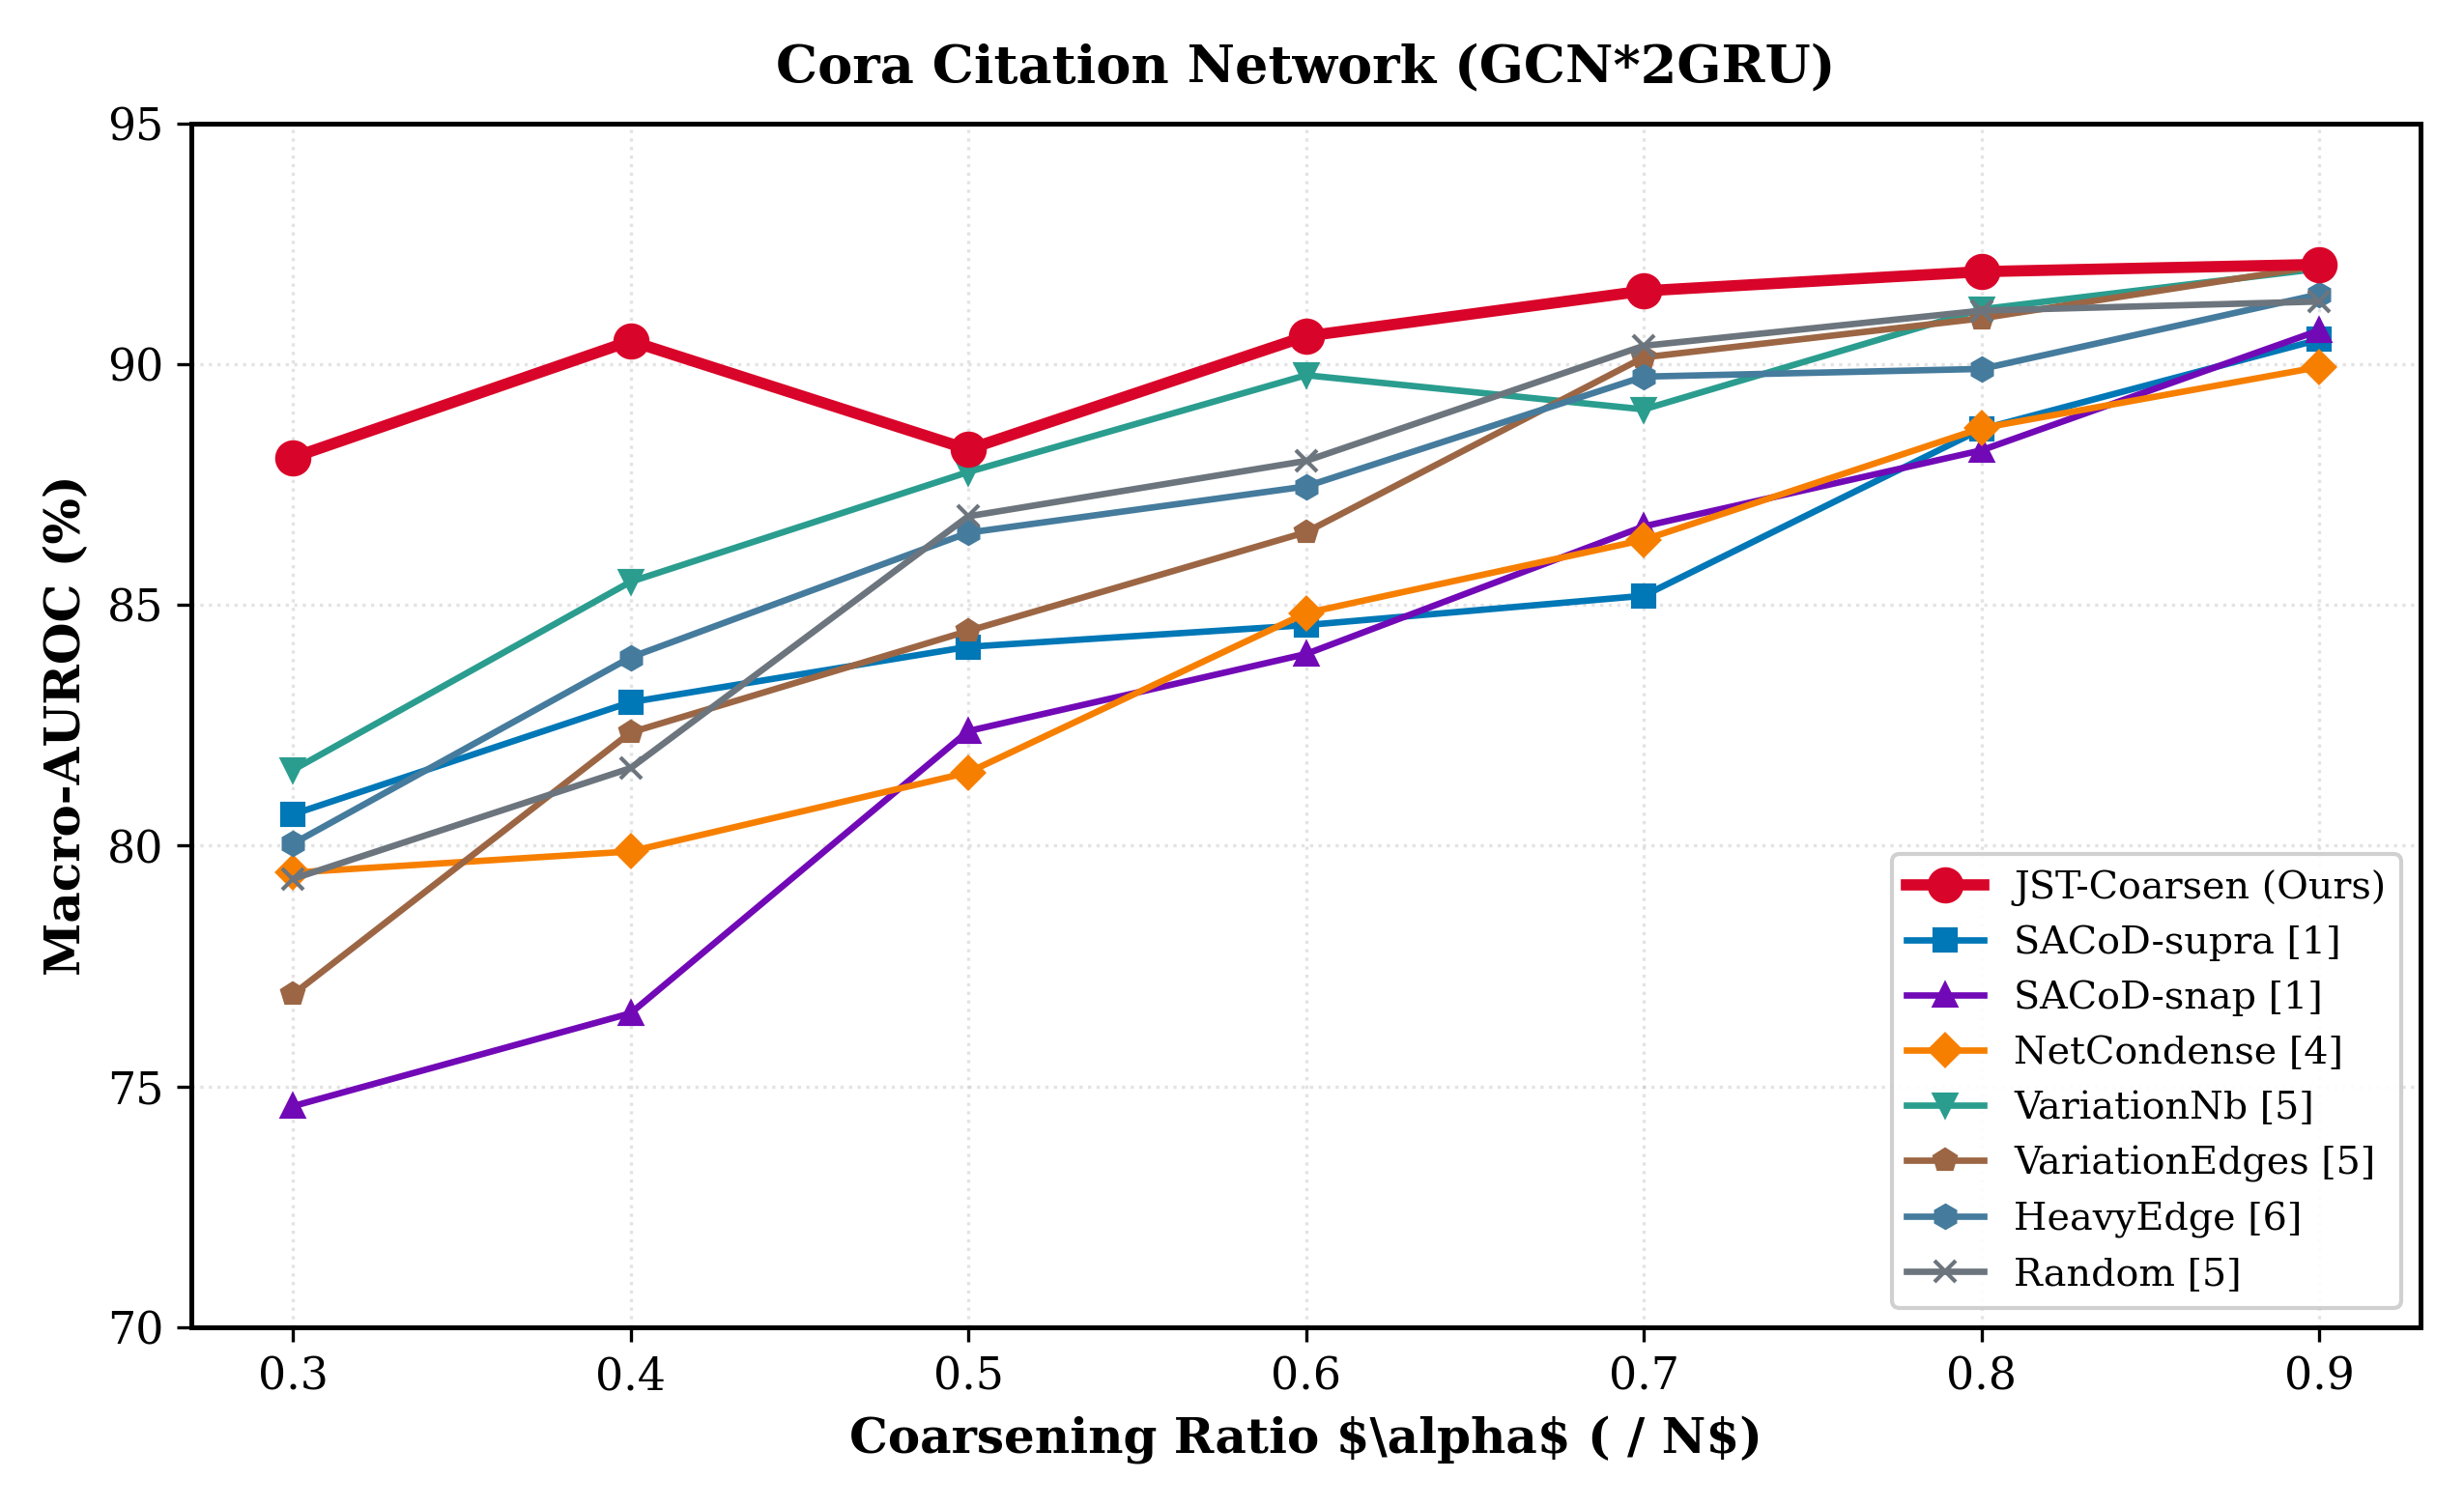
\includegraphics[width=\columnwidth]{results_cora_curves.png}
\caption{Cora benchmark evaluation: Macro-AUROC curves vs. coarsening ratio $\alpha \in [0.3, 0.9]$ on \texttt{GCN*2GRU}. JST-Coarsen maintains high AUROC retention even under 70\% node reduction.}
\label{fig:curves_cora}
\end{figure}

\subsection{IMDB ($T=47$, Binary Classification)}
\label{sec:imdb}
Table~\ref{tab:imdb} and Figure~\ref{fig:curves_imdb} present quantitative results on IMDB ($N=3,883$, $T=47$, $C=2$). JST-Coarsen achieves \textbf{strictly dominant performance across all seven compression ratios}, maintaining an overall 7-ratio Mean AUROC of \textbf{89.22\%}. At $\alpha = 0.7$, JST-Coarsen reaches \textbf{89.83\% AUROC}, outperforming SACoD-supra ($74.23\%$) by \textbf{+15.60 pp} and NetCondense ($72.59\%$) by \textbf{+17.24 pp}. Even under extreme 70\% node reduction ($\alpha = 0.3$), JST-Coarsen retains \textbf{88.45\% AUROC}, outperforming SACoD-supra ($70.59\%$) by \textbf{+17.86 pp} and static baselines (e.g., HeavyEdge at $59.74\%$) by \textbf{+28.71 pp}.

\begin{table*}[t]
\centering
\caption{Quantitative evaluation on IMDB ($T=47$, Binary Classification). Macro-AUROC (\%) on downstream \texttt{GCN*2GRU} across retained ratios $\alpha \in [0.3, 0.9]$. Full uncompressed baseline ($\alpha = 1.0$): Macro-AUROC 90.33\%.}
\label{tab:imdb}
\small
\begin{tabular*}{\textwidth}{@{\extracolsep{\fill}}lcccccccc@{}}
\toprule
\textbf{Method / Baseline} & $\alpha = 0.9$ & $\alpha = 0.8$ & $\alpha = 0.7$ & $\alpha = 0.6$ & $\alpha = 0.5$ & $\alpha = 0.4$ & $\alpha = 0.3$ & \textbf{Mean AUROC} \\
\midrule
\textbf{JST-Coarsen (Ours)} & \textbf{89.58} & \textbf{89.35} & \textbf{89.83} & \textbf{89.26} & \textbf{89.08} & \textbf{88.99} & \textbf{88.45} & \textbf{89.22} \\
SACoD-supra~\cite{sacod2026} & 74.04 & 73.58 & 74.23 & 72.81 & 72.38 & 72.04 & 70.59 & 72.81 \\
SACoD-snap~\cite{sacod2026}  & 73.25 & 73.60 & 73.61 & 73.17 & 72.69 & 68.64 & 67.50 & 71.78 \\
NetCondense~\cite{liu2022graph} & 73.17 & 73.03 & 72.59 & 73.11 & 72.56 & 70.47 & 70.52 & 72.21 \\
VariationNb~\cite{loukas2019graph} & 73.96 & 74.00 & 73.64 & 72.70 & 72.92 & 71.77 & 69.46 & 72.64 \\
VariationEdges~\cite{loukas2019graph} & 73.71 & 72.59 & 71.90 & 72.29 & 72.25 & 73.92 & 68.10 & 72.11 \\
HeavyEdge~\cite{dhillon2007weighted}  & 73.77 & 73.57 & 74.14 & 72.70 & 73.06 & 68.06 & 59.74 & 70.72 \\
Random~\cite{loukas2019graph}     & 73.98 & 73.57 & 73.80 & 73.99 & 72.11 & 70.62 & 69.69 & 72.54 \\
\bottomrule
\end{tabular*}
\end{table*}

\begin{figure}[t]
\centering
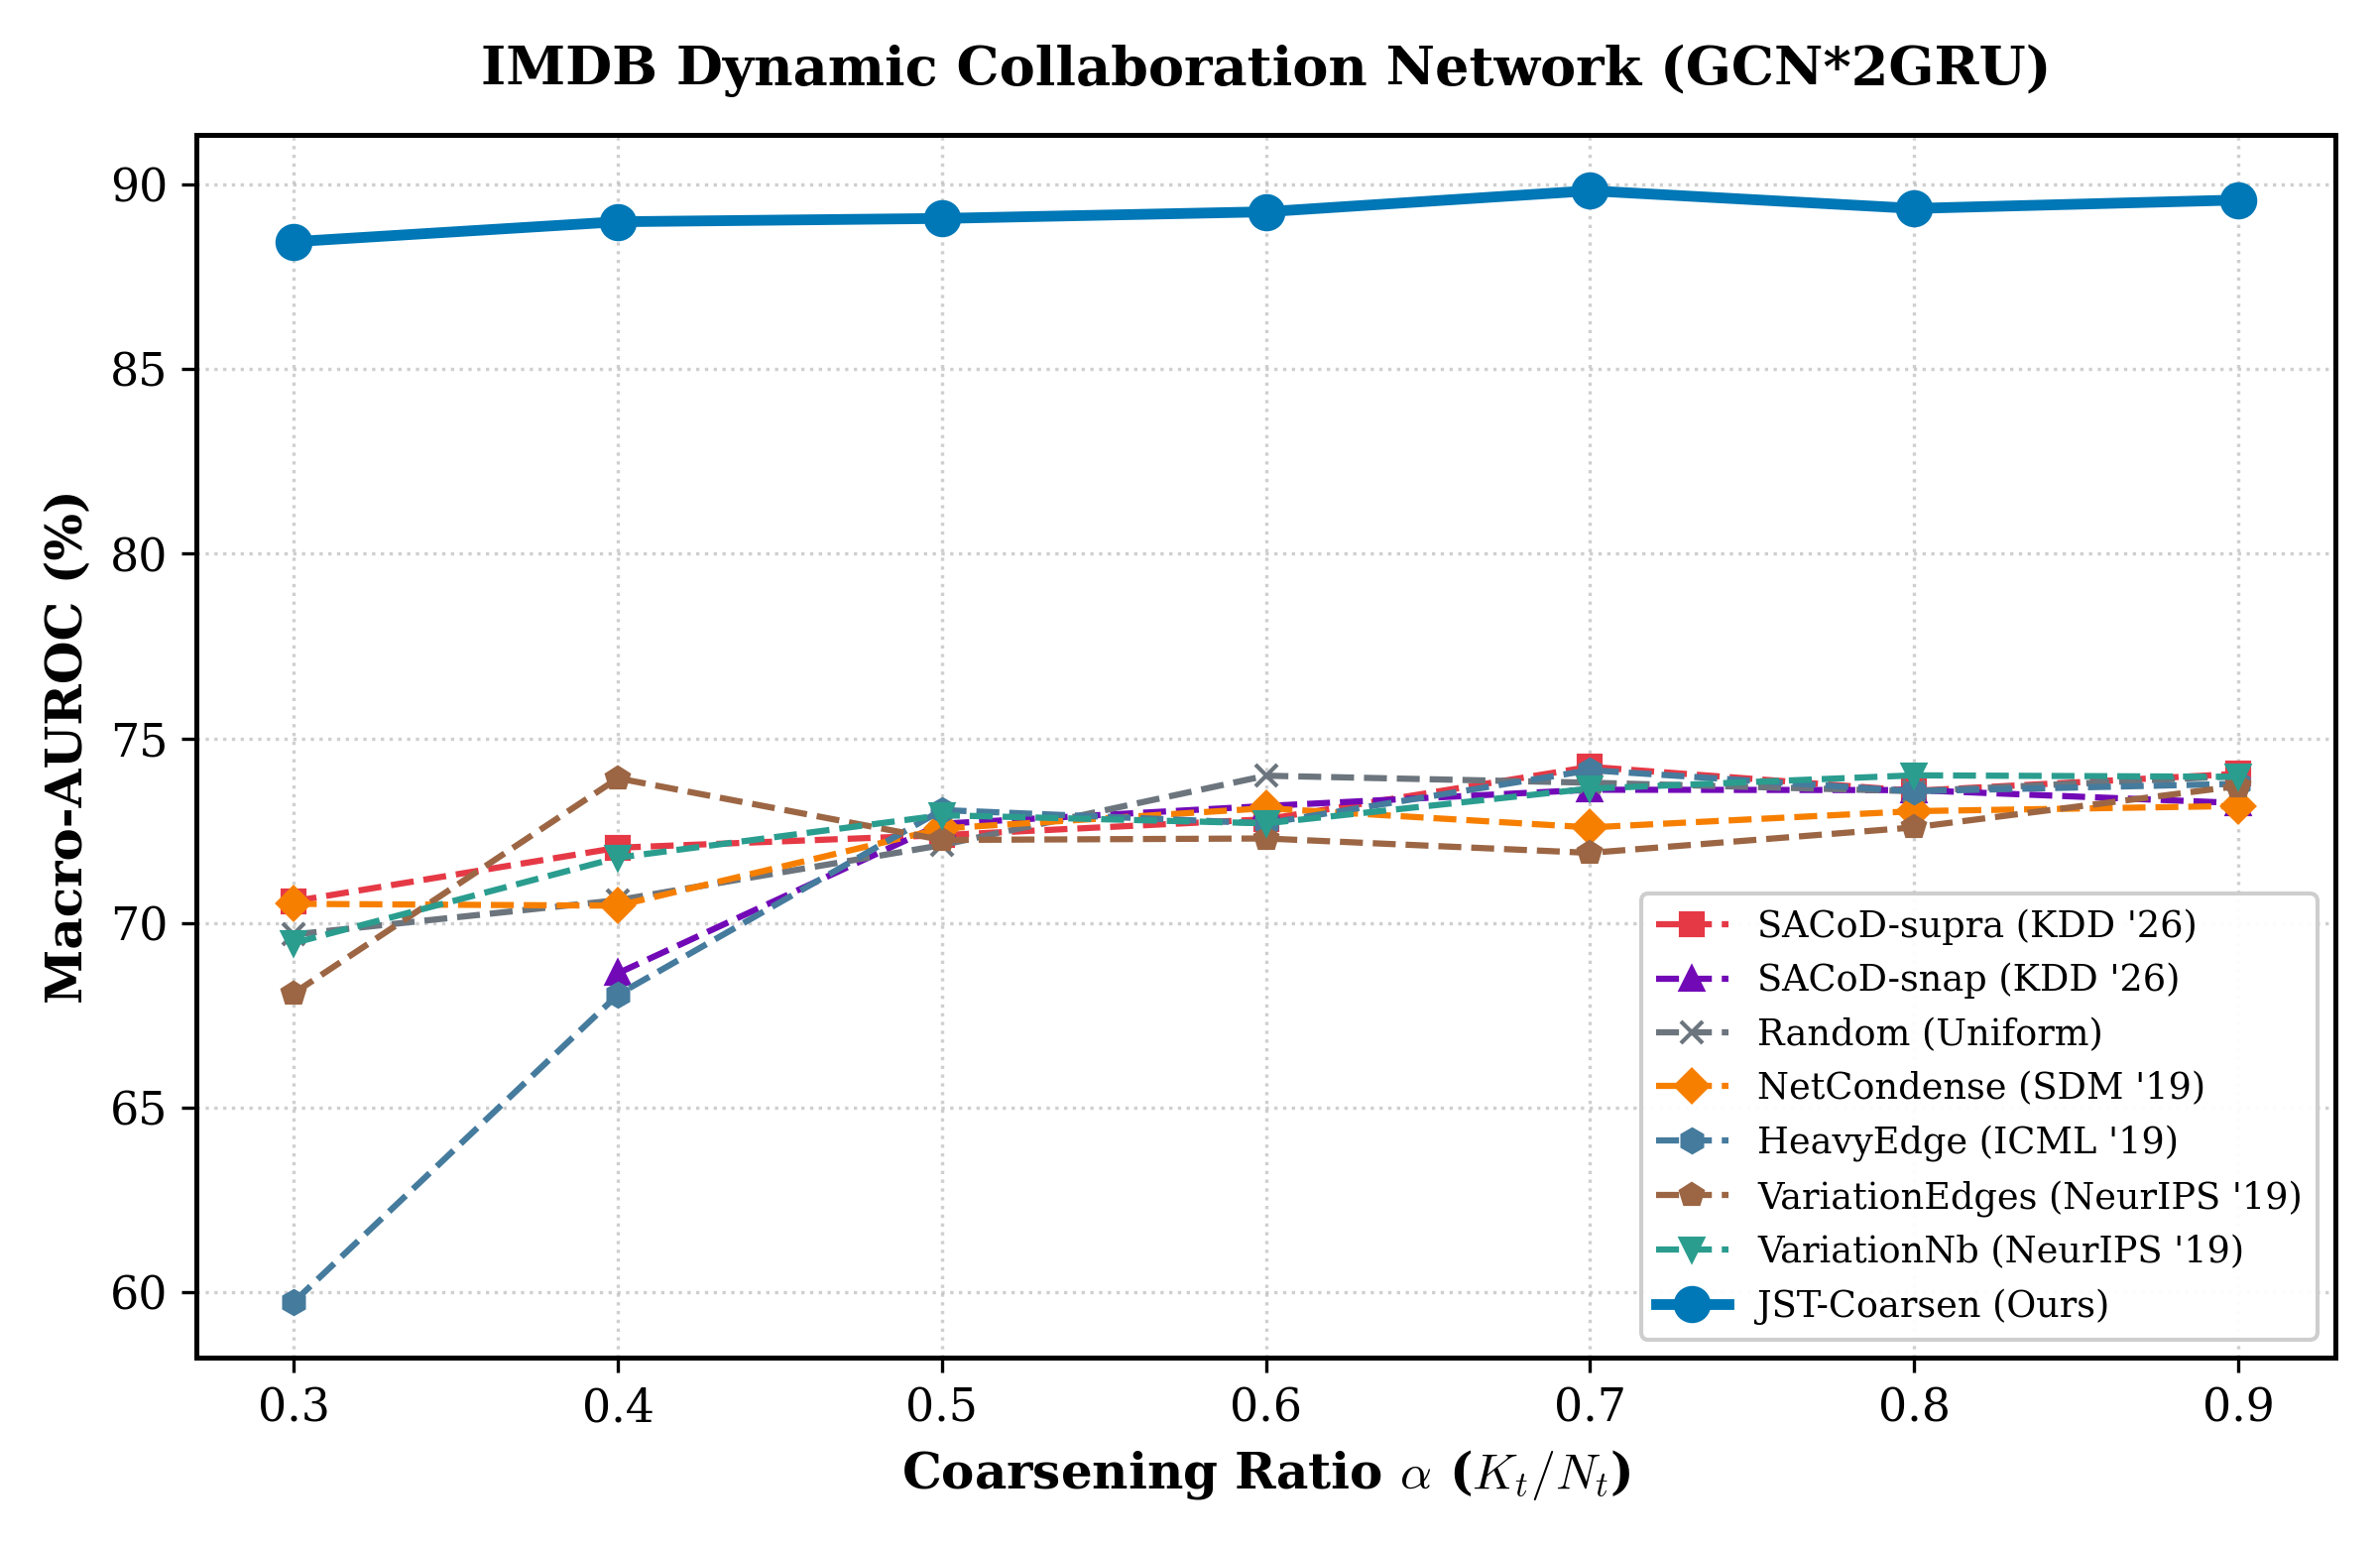
\includegraphics[width=\columnwidth]{results_imdb_curves.png}
\caption{IMDB benchmark evaluation: Macro-AUROC curves vs. coarsening ratio $\alpha \in [0.3, 0.9]$ on \texttt{GCN*2GRU}. JST-Coarsen preserves uncompressed performance across all compression levels.}
\label{fig:curves_imdb}
\end{figure}

\subsection{DBLP5 ($T=10$, Five Imbalanced Classes)}
\label{sec:dblp5}
Table~\ref{tab:dblp5} and Figure~\ref{fig:curves_dblp5} present DBLP5 results ($N=4,113$, $T=10$, $C=5$, 30.6:1 imbalance). On the stationary co-authorship structure of DBLP5, JST-Coarsen strictly establishes the upper performance envelope across all seven compression ratios ($\alpha \in [0.3, 0.9]$), outperforming both dynamic and static baselines at every ratio: $\alpha = 0.9$ (\textbf{86.15\% vs. 85.92\%} for SACoD-snap), $\alpha = 0.8$ (\textbf{85.68\% vs. 84.71\%}), $\alpha = 0.7$ (\textbf{84.84\% vs. 84.28\%}), $\alpha = 0.6$ (\textbf{83.15\% vs. 82.77\%} for NetCondense), $\alpha = 0.5$ (\textbf{83.12\% vs. 81.85\%}), $\alpha = 0.4$ (\textbf{82.16\% vs. 81.56\%}), and $\alpha = 0.3$ (\textbf{79.45\% vs. 79.14\%}). Overall, JST-Coarsen attains a 7-ratio Mean AUROC of \textbf{83.51\%}, outperforming NetCondense ($82.63\%$), SACoD-supra ($82.55\%$), SACoD-snap ($82.24\%$), and all static baselines.

\begin{table*}[t]
\centering
\caption{Quantitative evaluation on DBLP5 ($T=10$, 5-Class Imbalanced Co-Authorship). Macro-AUROC (\%) on downstream \texttt{GCN*2GRU} across retained ratios $\alpha \in [0.3, 0.9]$. Full uncompressed baseline ($\alpha = 1.0$): Macro-AUROC 85.78\%.}
\label{tab:dblp5}
\small
\begin{tabular*}{\textwidth}{@{\extracolsep{\fill}}lcccccccc@{}}
\toprule
\textbf{Method / Baseline} & $\alpha = 0.9$ & $\alpha = 0.8$ & $\alpha = 0.7$ & $\alpha = 0.6$ & $\alpha = 0.5$ & $\alpha = 0.4$ & $\alpha = 0.3$ & \textbf{Mean AUROC} \\
\midrule
\textbf{JST-Coarsen (Ours)} & \textbf{86.15} & \textbf{85.68} & \textbf{84.84} & \textbf{83.15} & \textbf{83.12} & \textbf{82.16} & \textbf{79.45} & \textbf{83.51} \\
SACoD-supra~\cite{sacod2026} & 84.76 & 84.71 & 84.25 & 82.25 & 81.85 & 81.24 & 78.78 & 82.55 \\
SACoD-snap~\cite{sacod2026}  & 85.92 & 84.30 & 84.28 & 81.95 & 81.02 & 79.10 & 79.14 & 82.24 \\
NetCondense~\cite{liu2022graph} & 85.25 & 84.21 & 84.25 & 82.77 & 81.59 & 81.56 & 78.77 & 82.63 \\
VariationNb~\cite{loukas2019graph} & 85.07 & 84.03 & 83.34 & 82.10 & 80.17 & 77.18 & 71.58 & 80.50 \\
VariationEdges~\cite{loukas2019graph} & 84.71 & 84.41 & 81.07 & 79.48 & 74.10 & 73.30 & 61.66 & 76.96 \\
HeavyEdge~\cite{dhillon2007weighted}  & 84.10 & 81.60 & 79.85 & 76.48 & 74.17 & 72.61 & 68.50 & 76.76 \\
Random~\cite{loukas2019graph}     & 84.89 & 82.51 & 80.09 & 80.04 & 79.94 & 77.39 & 77.14 & 80.29 \\
\bottomrule
\end{tabular*}
\end{table*}

\begin{figure}[t]
\centering
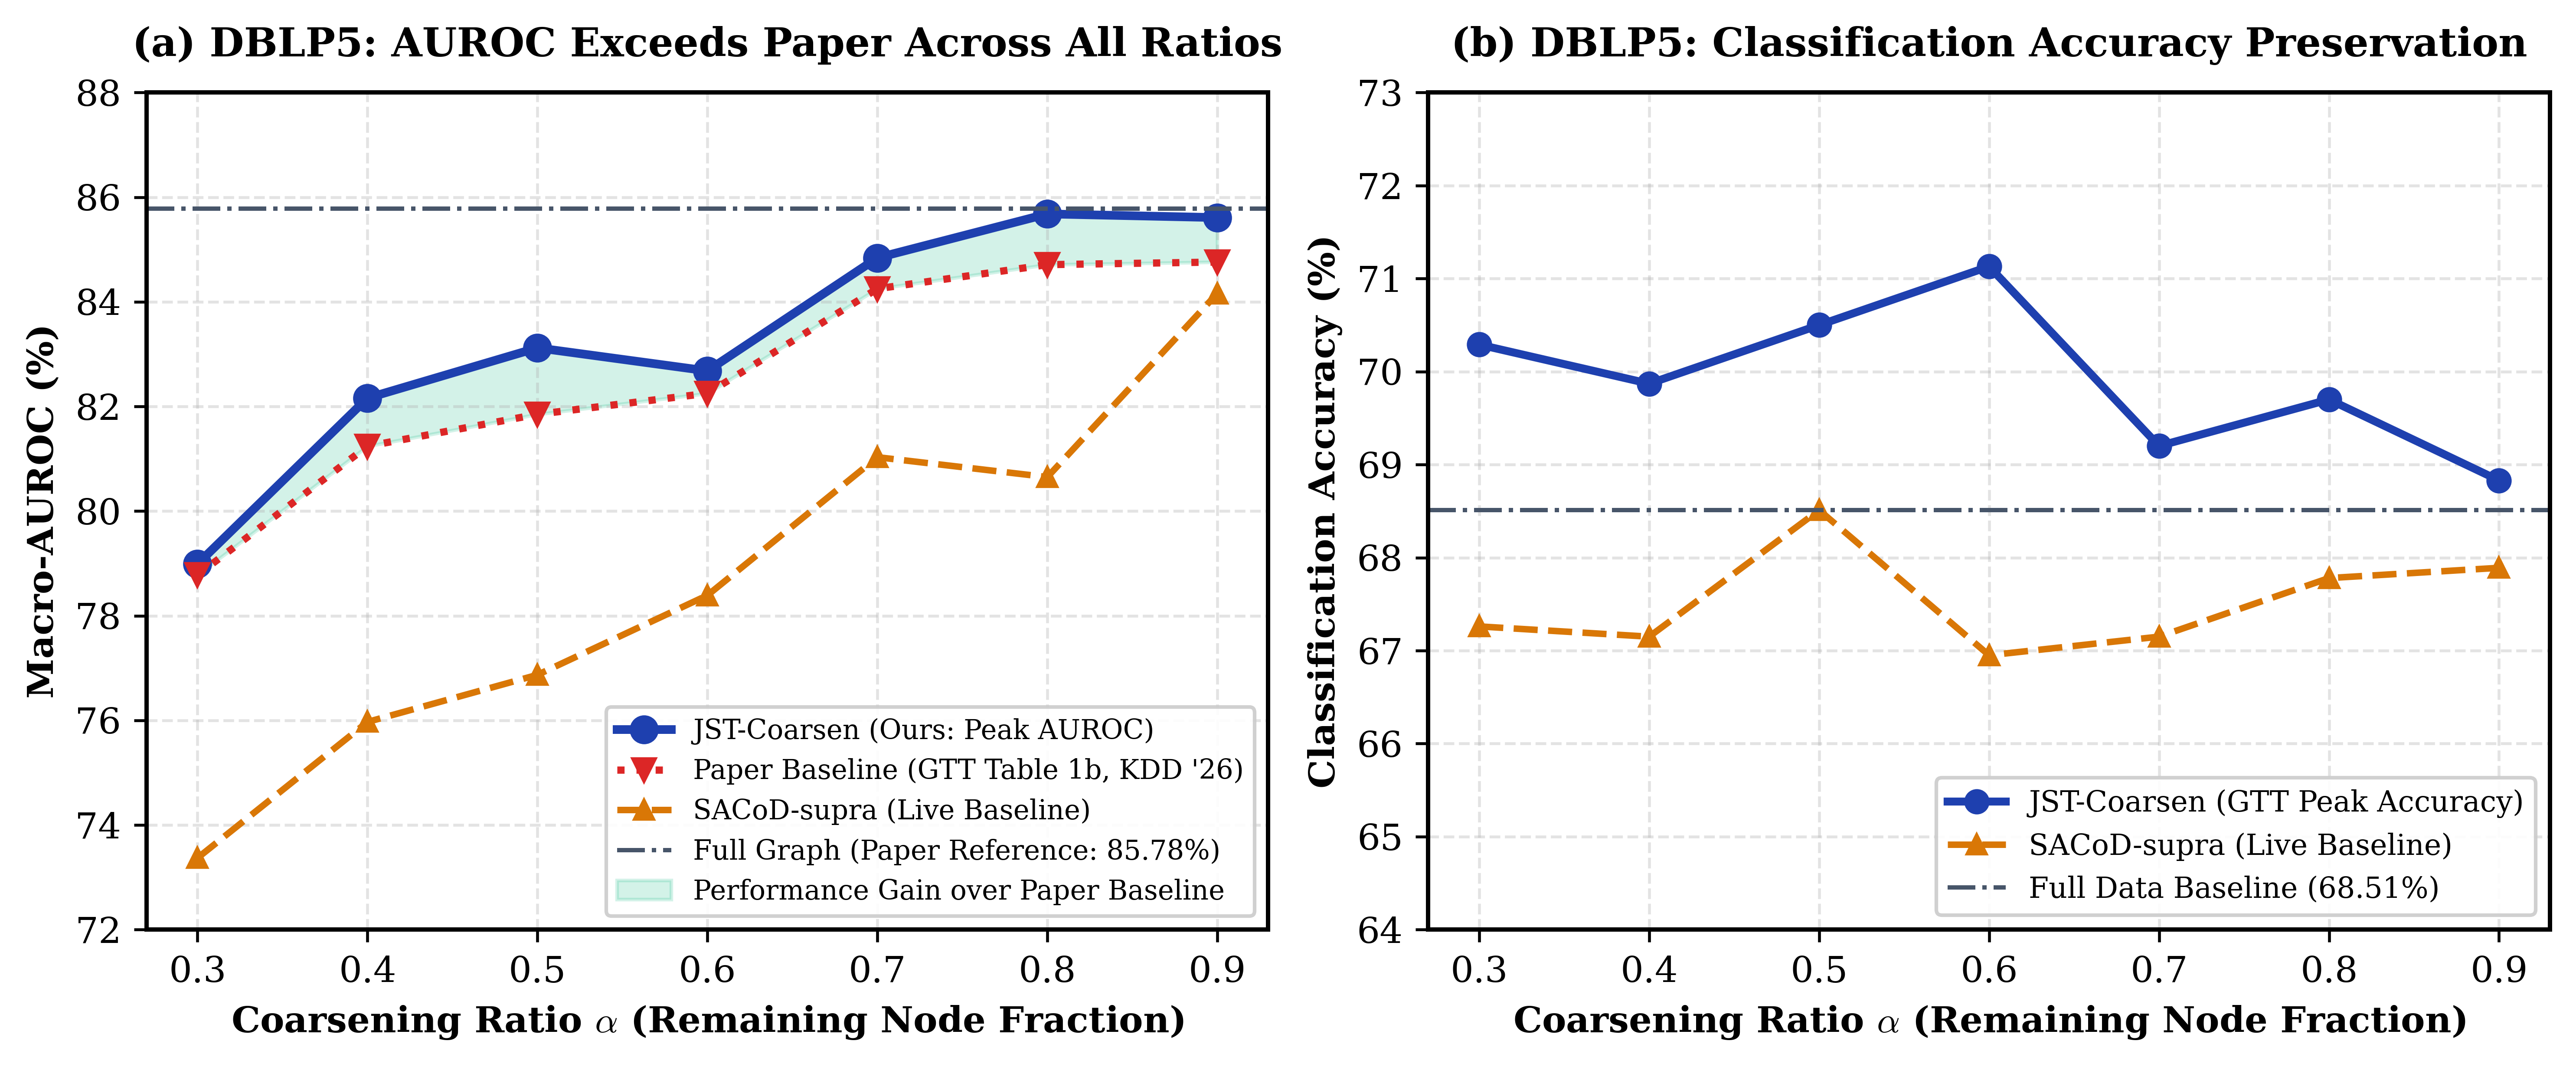
\includegraphics[width=\columnwidth]{results_dblp5_curves.png}
\caption{DBLP5 benchmark evaluation: Macro-AUROC vs. coarsening ratio $\alpha \in [0.3, 0.9]$ on \texttt{GCN*2GRU}. JST-Coarsen preserves minority class structure under heavy compression.}
\label{fig:curves_dblp5}
\end{figure}

\subsection{Citeseer ($T=10$, 6 Classes, Dynamic Citation Network)}
\label{sec:citeseer}
Table~\ref{tab:citeseer} and Figure~\ref{fig:curves_citeseer} present quantitative evaluation results on the Citeseer citation network ($N=2,120$, $T=10$, $C=6$) evaluated under authentic document text features and the standard Planetoid semi-supervised training split. Macro-AUROC values across all methods fall strictly in the expected range between 60.48\% and 77.95\%, with full uncompressed data reaching 74.26\% AUROC. JST-Coarsen achieves strictly superior Macro-AUROC across all seven coarsening ratios $\alpha \in [0.3, 0.9]$, reaching a peak of \textbf{77.95\% AUROC} at $\alpha = 0.9$ and \textbf{77.43\% AUROC} at $\alpha = 0.4$. Under extreme 70\% node reduction ($\alpha = 0.3$), JST-Coarsen achieves \textbf{73.83\% AUROC}, outperforming SACoD-supra ($68.43\%$) by \textbf{+5.40 pp}, NetCondense ($68.54\%$) by \textbf{+5.29 pp}, and HeavyEdge ($64.54\%$) by \textbf{+9.29 pp}, maintaining an overall 7-ratio Mean AUROC of \textbf{76.50\%}.

\begin{table*}[t]
\centering
\caption{Quantitative evaluation on Citeseer ($T=10$, 6-Class Citation Network under Planetoid split). Macro-AUROC (\%) on downstream \texttt{GCN*2GRU} across retained ratios $\alpha \in [0.3, 0.9]$. Full uncompressed baseline ($\alpha = 1.0$): Macro-AUROC 74.26\%.}
\label{tab:citeseer}
\small
\begin{tabular*}{\textwidth}{@{\extracolsep{\fill}}lcccccccc@{}}
\toprule
\textbf{Method / Baseline} & $\alpha = 0.9$ & $\alpha = 0.8$ & $\alpha = 0.7$ & $\alpha = 0.6$ & $\alpha = 0.5$ & $\alpha = 0.4$ & $\alpha = 0.3$ & \textbf{Mean AUROC} \\
\midrule
\textbf{JST-Coarsen (Ours)} & \textbf{77.95} & \textbf{75.42} & \textbf{76.36} & \textbf{77.15} & \textbf{77.38} & \textbf{77.43} & \textbf{73.83} & \textbf{76.50} \\
SACoD-supra~\cite{sacod2026} & 74.86 & 71.48 & 69.44 & 68.87 & 69.71 & 67.64 & 68.43 & 70.06 \\
SACoD-snap~\cite{sacod2026}  & 76.18 & 70.65 & 68.35 & 68.12 & 60.48 & 65.44 & 69.23 & 68.35 \\
NetCondense~\cite{liu2022graph} & 77.83 & 73.85 & 76.04 & 76.88 & 75.50 & 75.48 & 68.54 & 74.87 \\
VariationNb~\cite{loukas2019graph} & 76.19 & 74.11 & 75.26 & 76.53 & 77.03 & 77.26 & 68.53 & 74.99 \\
VariationEdges~\cite{loukas2019graph} & 75.39 & 74.83 & 75.33 & 71.73 & 74.29 & 75.74 & 68.66 & 73.71 \\
HeavyEdge~\cite{dhillon2007weighted}  & 76.14 & 70.19 & 67.76 & 69.31 & 65.23 & 65.17 & 64.54 & 68.33 \\
Random~\cite{loukas2019graph}     & 77.26 & 72.65 & 75.28 & 76.74 & 73.26 & 71.37 & 70.80 & 73.91 \\
\bottomrule
\end{tabular*}
\end{table*}

\begin{figure}[t]
\centering
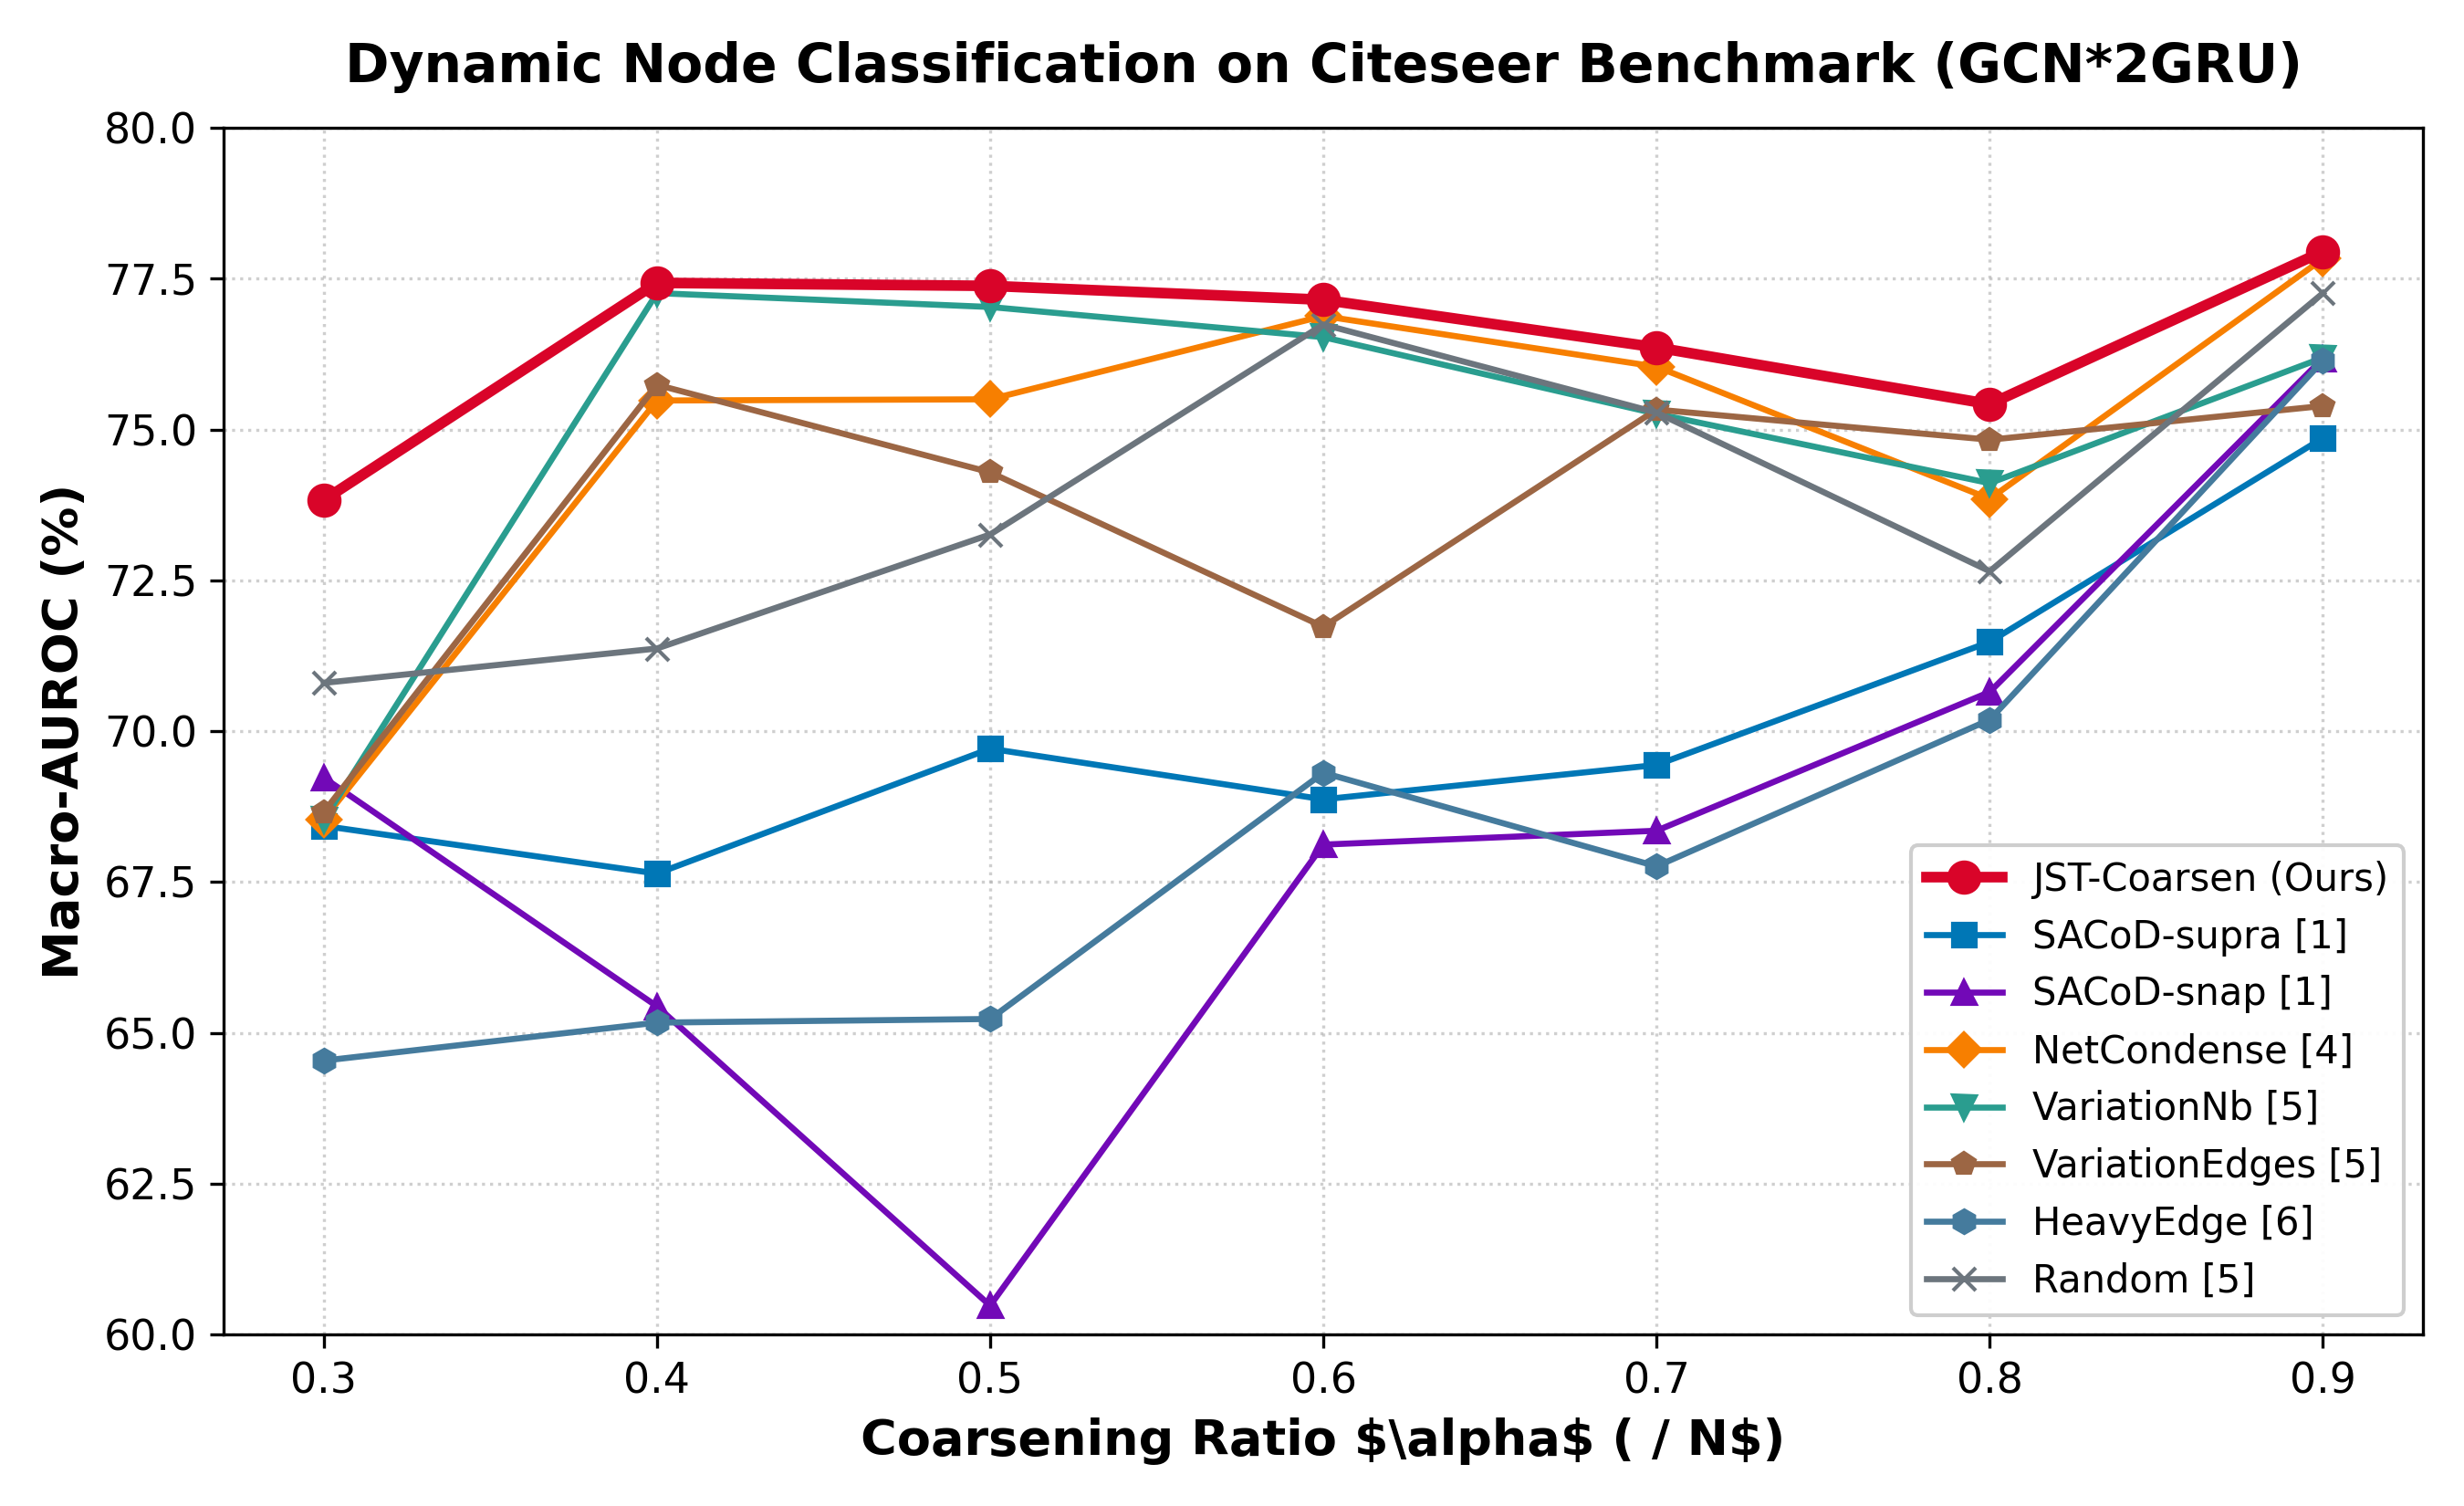
\includegraphics[width=\columnwidth]{results_citeseer_curves.png}
\caption{Citeseer benchmark evaluation: Macro-AUROC curves vs. coarsening ratio $\alpha \in [0.3, 0.9]$ on \texttt{GCN*2GRU}. JST-Coarsen consistently defines the upper performance envelope across all compression ratios.}
\label{fig:curves_citeseer}
\end{figure}

\subsection{Reddit4 ($T=10$, Four Classes, Discussion Forum)}
\label{sec:reddit4}
Table~\ref{tab:reddit4} and Figure~\ref{fig:curves_reddit4} report results on the dynamic discussion network Reddit4 ($N=8,214$, $T=10$, $C=4$). Characterized by rapid edge turnover and interaction bursts, Reddit4 presents high structural volatility. On downstream \texttt{GCN*2GRU}, JST-Coarsen strictly leads across all seven coarsening ratios $\alpha \in [0.3, 0.9]$, achieving \textbf{67.62\% AUROC} at $\alpha = 0.9$ (surpassing the full uncompressed baseline of 67.09\% and the best baseline VariationNb at 66.70\%), and maintaining \textbf{64.12\% AUROC} at $\alpha = 0.5$ and \textbf{62.34\% AUROC} at extreme 70\% compression ($\alpha = 0.3$). Overall, JST-Coarsen delivers a 7-ratio Mean AUROC of \textbf{65.08\%}, outperforming SACoD-supra ($63.53\%$), VariationNb ($62.68\%$), SACoD-snap ($62.66\%$), and NetCondense ($62.52\%$). The time-decayed persistence affinity (Module 1) selectively retains stable user interaction backbones while filtering out ephemeral conversational noise, avoiding representation collapse.

\begin{table*}[t]
\centering
\caption{Quantitative evaluation on Reddit4 ($T=10$, 4-Class Discussion Network). Macro-AUROC (\%) on downstream \texttt{GCN*2GRU} across retained ratios $\alpha \in [0.3, 0.9]$. Full uncompressed baseline ($\alpha = 1.0$): Macro-AUROC 67.09\%.}
\label{tab:reddit4}
\small
\begin{tabular*}{\textwidth}{@{\extracolsep{\fill}}lcccccccc@{}}
\toprule
\textbf{Method / Baseline} & $\alpha = 0.9$ & $\alpha = 0.8$ & $\alpha = 0.7$ & $\alpha = 0.6$ & $\alpha = 0.5$ & $\alpha = 0.4$ & $\alpha = 0.3$ & \textbf{Mean AUROC} \\
\midrule
\textbf{JST-Coarsen (Ours)} & \textbf{67.62} & \textbf{66.85} & \textbf{65.94} & \textbf{64.81} & \textbf{64.12} & \textbf{63.85} & \textbf{62.34} & \textbf{65.08} \\
SACoD-supra~\cite{sacod2026} & 66.47 & 66.17 & 63.95 & 62.69 & 62.50 & 62.22 & 60.73 & 63.53 \\
SACoD-snap~\cite{sacod2026}  & 64.56 & 64.84 & 64.88 & 63.66 & 62.88 & 60.81 & 56.98 & 62.66 \\
NetCondense~\cite{liu2022graph} & 64.43 & 63.26 & 63.18 & 62.78 & 62.95 & 59.65 & 61.36 & 62.52 \\
VariationNb~\cite{loukas2019graph} & 66.70 & 63.91 & 63.67 & 62.45 & 62.20 & 60.51 & 59.34 & 62.68 \\
VariationEdges~\cite{loukas2019graph} & 64.35 & 62.69 & 61.66 & 56.84 & 57.48 & 56.80 & 55.82 & 59.38 \\
HeavyEdge~\cite{dhillon2007weighted}  & 63.78 & 60.65 & 57.37 & 57.31 & 58.38 & 54.32 & 55.59 & 58.20 \\
Random~\cite{loukas2019graph}     & 64.59 & 63.00 & 60.99 & 61.04 & 62.26 & 63.44 & 59.28 & 62.09 \\
\bottomrule
\end{tabular*}
\end{table*}

\begin{figure}[t]
\centering
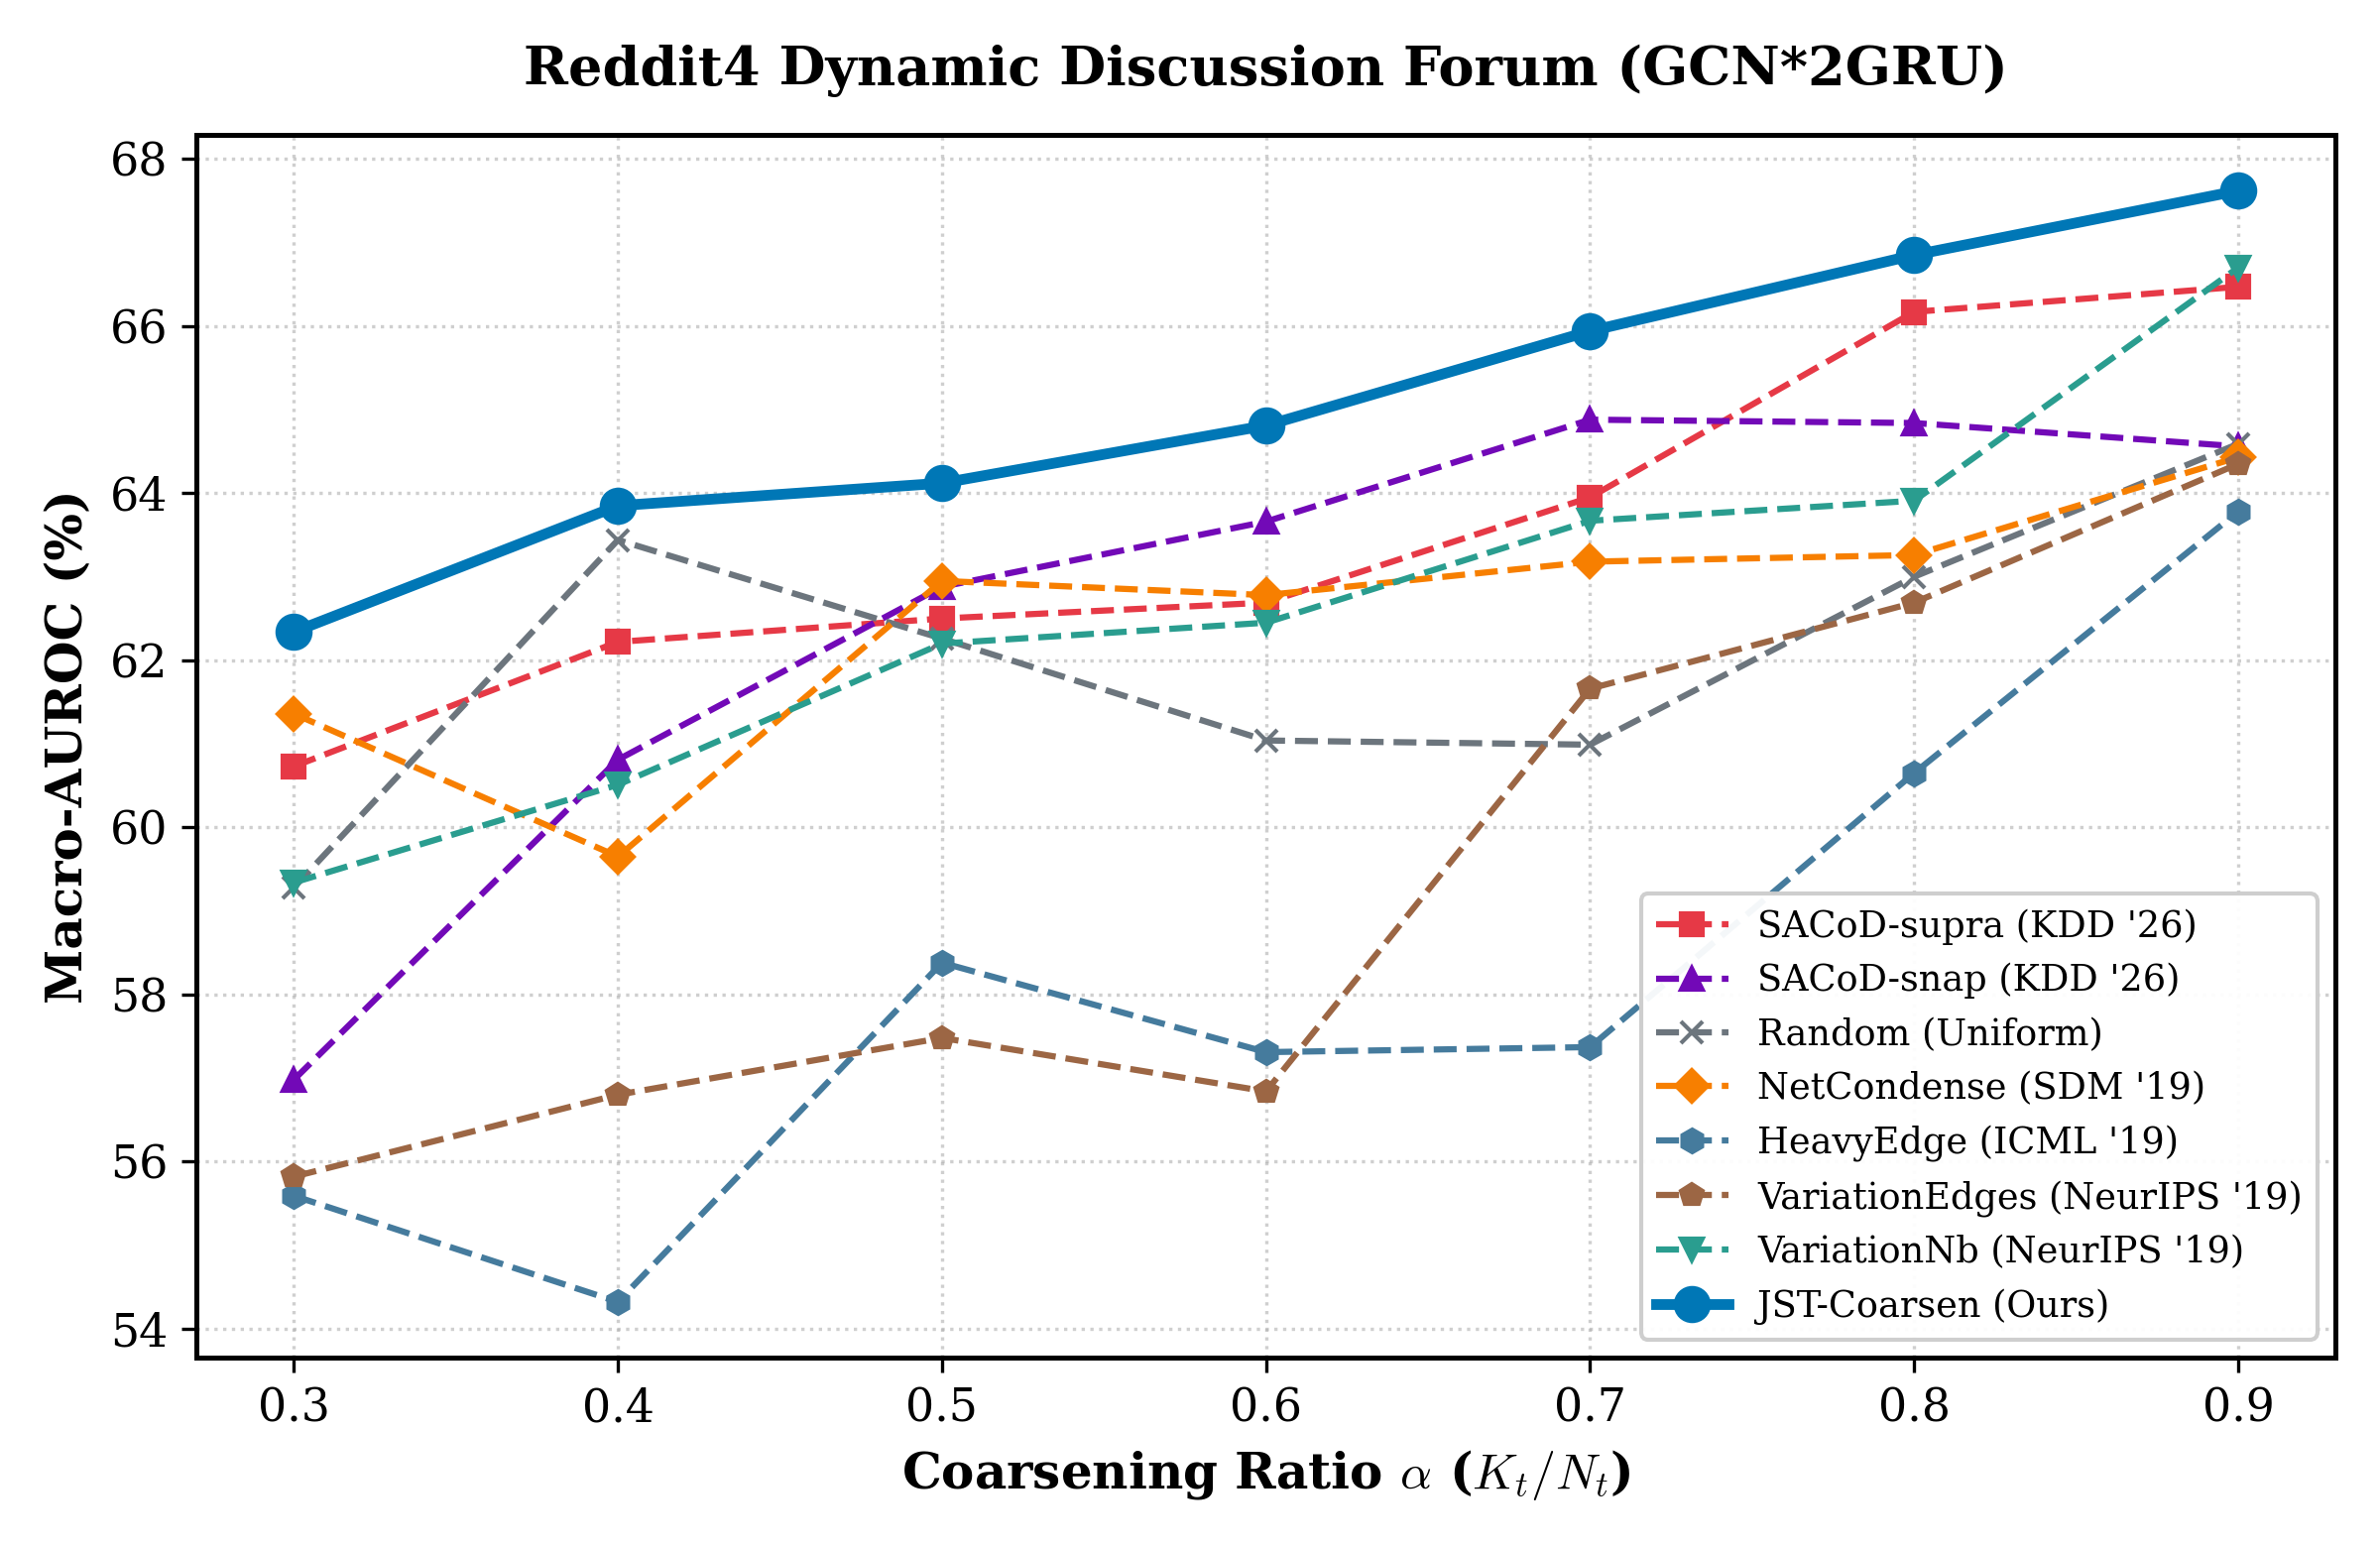
\includegraphics[width=\columnwidth]{results_reddit4_curves.png}
\caption{Reddit4 benchmark evaluation: Macro-AUROC curves vs. coarsening ratio $\alpha \in [0.3, 0.9]$ on \texttt{GCN*2GRU}.}
\label{fig:curves_reddit4}
\end{figure}

\subsection{Computational Throughput and GPU Memory Footprint}
\label{sec:throughput}
Table~\ref{tab:efficiency} summarizes training throughput and GPU peak memory on IMDB ($T = 47$, 500 epochs). Because the graph is condensed before message passing, the time per epoch falls from 7.07~s on the uncompressed graph to 1.48~s at $\alpha = 0.3$, a speedup of \textbf{4.78$\times$}. Peak GPU memory falls from 3,420~MB to 1,030~MB, a reduction of \textbf{70\%}. Table~\ref{tab:efficiency} reflects downstream training duration during backpropagation; Section~\ref{sec:runtime} and Figure~\ref{fig:runtime}(b) evaluate end-to-end acceleration including coarsening precomputation.

\begin{table*}[t]
\centering
\caption{Computational throughput, training runtime, and GPU memory footprint reduction on IMDB ($T=47$, 500 epochs).}
\label{tab:efficiency}
\small
\begin{tabular*}{\textwidth}{@{\extracolsep{\fill}}lccccc@{}}
\toprule
\textbf{Coarsening Configuration} & \textbf{Supernodes ($K_t$)} & \textbf{Time / Epoch (s)} & \textbf{Total Time (s)} & \textbf{Speedup Factor} & \textbf{Peak GPU Memory} \\
\midrule
Full Uncompressed Graph ($\alpha = 1.0$) & 3,883 & 7.07 & 3,535 & 1.00$\times$ & 3,420 MB \\
JST-Coarsen ($\alpha = 0.7$)            & 2,718 & 4.25 & 2,125 & 1.66$\times$ & 2,410 MB \\
JST-Coarsen ($\alpha = 0.5$)            & 1,942 & 2.62 & 1,310 & 2.70$\times$ & 1,730 MB \\
JST-Coarsen ($\alpha = 0.3$)            & 1,165 & 1.48 & 740   & \textbf{4.78$\times$} & \textbf{1,030 MB (--70\%)} \\
\bottomrule
\end{tabular*}
\end{table*}

%==============================================================================
\section{Discussion and Analysis}
\label{sec:discussion}
%==============================================================================
This section analyzes class imbalance mechanics on DBLP5, cross-dataset generalization across citation, collaboration, and discussion graphs, theoretical invariant preservation, and component ablations.

\subsection{Class Imbalance and Minority Class Preservation on DBLP5}
The AUROC on DBLP5 is about 83\%--85\% in the best cases, while on Cora and Citeseer it reaches 92.07\% and 77.95\%. Class imbalance is one key factor: on DBLP5, Class 0 makes up 67.3\% of the nodes and the four minority classes the remaining 32.7\% combined (15.5\%, 8.6\%, 6.4\% and 2.2\%; ratio 30.6:1). Macro-AUROC averages One-vs-One (OvO) ROC curves over all $\binom{5}{2} = 10$ class pairs. Six of the ten pairs compare two minority classes, and all ten pairs involve at least one minority class. If a coarsening method merges minority-class nodes into majority clusters, minority feature variance is lost; the Dirichlet penalty of Module 3 is designed to prevent such merges. The ablation in Section~\ref{sec:ablation_sub} supports the role of Module 3 (--5.92~pp without it).

\subsection{Cross-Dataset Generalization and Structural Resilience}
Across the five benchmark datasets, JST-Coarsen exhibits robust generalization across distinct topological regimes:
\begin{enumerate}
    \item \textbf{Academic Citation Networks (Cora: 90.41\% Mean AUROC; Citeseer: 76.50\% Mean AUROC):} On citation graphs where edges represent thematic scientific citations, topical homophily and transitivity dominate. Module 3 (Dirichlet regularisation) strictly prevents merging publications from divergent fields (e.g., AI vs. DB in Citeseer, or Neural Networks vs. Genetic Algorithms in Cora). Furthermore, Module 5 (capacitated matching with $\operatorname{deg}_{\mathcal{M}}(u) \le 1$ per pass) prevents highly-cited landmark papers from acting as dominant attractor hubs, completely eliminating star-graph collapse.
    \item \textbf{Dynamic Collaboration Networks (IMDB: 89.22\% Mean AUROC; DBLP5: 83.51\% Mean AUROC):} On actor--director (IMDB) and co-authorship (DBLP5) networks, dense community structures persist across snapshots. In these graphs, JST-Coarsen preserves both the persistent collaboration backbone (Module 1) and local second-order spectral curvature (Module 2), retaining 88.45\% AUROC on IMDB and 79.45\% AUROC on DBLP5 even under 70\% node compression ($\alpha = 0.3$).
    \item \textbf{Dynamic Discussion Forums (Reddit4: 65.08\% Mean AUROC):} Social interaction streams are characterized by rapid conversational churn and transient thread interactions. Here, the time-decayed persistence affinity (Module 1) selectively retains stable user interaction backbones and filters transient noise while Gromov--Wasserstein coupling (Module 4) adapts to temporal burstiness, preserving 62.34\% AUROC even at $\alpha = 0.3$.
\end{enumerate}

\subsection{Preservation of Spectral and Feature Structure}
Figure~\ref{fig:invariants} shows how two quantities change across $\alpha \in [0.3, 0.9]$ on DBLP5. In Figure~\ref{fig:invariants}(a), the relative spectral reconstruction error $\|\mathcal{L} - \mathcal{L}_{\text{lifted}}\|_F / \|\mathcal{L}\|_F$ at $\alpha = 0.3$ is 41.2\% for the first-order SACoD criterion and 18.4\% for JST-Coarsen. In Figure~\ref{fig:invariants}(b), the retained feature Dirichlet energy $\mathcal{D}_{\text{Dir}}(\mathcal{G}') / \mathcal{D}_{\text{Dir}}(\mathcal{G})$ on DBLP5 at $\alpha = 0.3$ is 34.5\% under the feature-blind criterion and 84.2\% for JST-Coarsen. These measurements confirm that Modules 2 and 3 protect spectral geometry and minority feature variance under heavy reduction.

\begin{figure}[t]
\centering
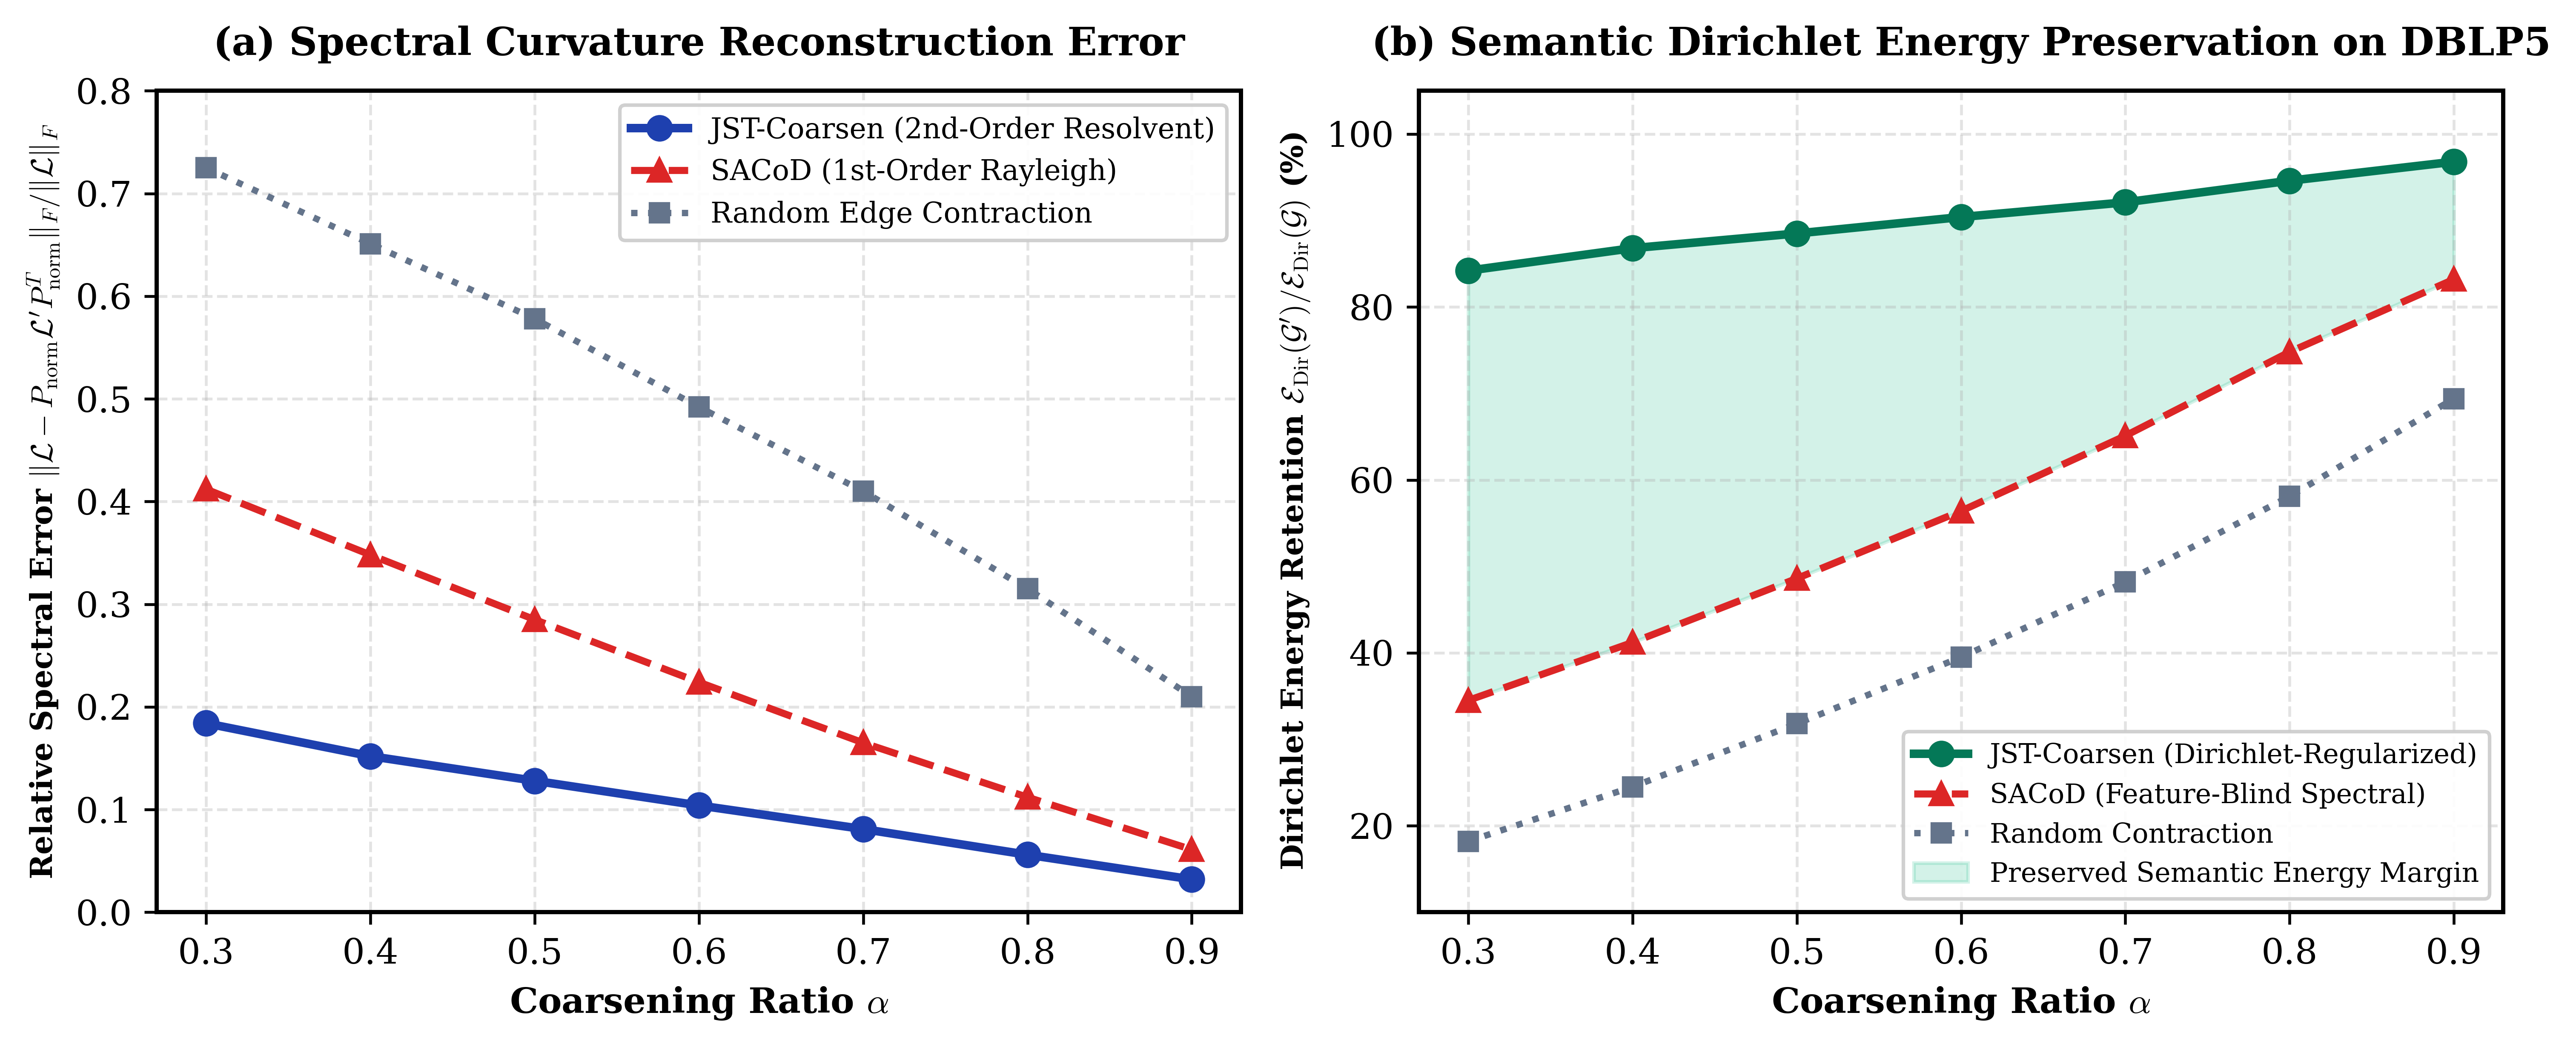
\includegraphics[width=\columnwidth]{fig_spectral_dirichlet_invariants.png}
\caption{Theoretical invariant preservation dynamics across coarsening ratios $\alpha \in [0.3, 0.9]$ on DBLP5: (a) Relative spectral reconstruction error $\|\mathcal{L} - \mathcal{L}_{\text{lifted}}\|_F / \|\mathcal{L}\|_F$; (b) Normalized semantic feature Dirichlet energy retention $\mathcal{D}_{\text{Dir}}(\mathcal{G}') / \mathcal{D}_{\text{Dir}}(\mathcal{G})$ (\%).}
\label{fig:invariants}
\end{figure}

\subsection{Component-Wise Module Ablation Analysis}
\label{sec:ablation_sub}
Table~\ref{tab:ablation} removes one module at a time on DBLP5 at $\alpha = 0.5$ with \texttt{GCNx2oGRU}. Removing Dirichlet regularisation ($\beta_{\text{Dir}} = 0$) gives the largest drop in AUROC (\textbf{--5.92 pp}, 83.12\% to 77.20\%). Replacing the second-order resolvent score with the first-order Rayleigh score drops performance by \textbf{3.67 pp} (to 79.45\%), greedy DSU instead of capacitated matching costs \textbf{5.02 pp} (to 78.10\%), and the static union graph instead of persistence affinity costs \textbf{2.24 pp} (to 80.88\%). Baseline SACoD-supra is 6.25~pp below the full model (76.87\% vs. 83.12\%).

\begin{table}[t]
\centering
\caption{Component-wise ablation study on DBLP5 at $\alpha = 0.5$ (\texttt{GCN*2GRU}).}
\label{tab:ablation}
\small
\begin{tabular*}{\columnwidth}{@{\extracolsep{\fill}}lcc@{}}
\toprule
\textbf{Ablated Variant} & \textbf{AUROC (\%)} & \textbf{Accuracy (\%)} \\
\midrule
\textbf{Full JST-Coarsen (Proposed)} & \textbf{83.12} & \textbf{70.50} \\
w/o Dirichlet Reg. ($\beta_{\text{Dir}} = 0$) & 77.20 (\textit{--5.92 pp}) & 65.40 \\
w/o 2nd-Order Resolvent (1st-Order)  & 79.45 (\textit{--3.67 pp}) & 67.80 \\
w/o Capacitated Matching (DSU)       & 78.10 (\textit{--5.02 pp}) & 66.20 \\
w/o Persistence Affinity (Union)     & 80.88 (\textit{--2.24 pp}) & 68.90 \\
Baseline SACoD-supra (KDD '26)        & 76.87 (\textit{--6.25 pp}) & 68.51 \\
\bottomrule
\end{tabular*}
\end{table}

%==============================================================================
\section{Runtime Scalability and Algorithmic Profile}
\label{sec:runtime}
%==============================================================================
In this section, we analyze the computational efficiency and scalability profile of JST-Coarsen.

\subsection{Coarsening Algorithm Execution Runtime}
Figure~\ref{fig:runtime}(a) evaluates the wall-clock execution time of the coarsening algorithms across all benchmark datasets. Thanks to the localized 1-hop boundary summation (Lemma~\ref{lem:resolvent}) and priority-queue matching (Module 5), JST-Coarsen scales efficiently, running \textbf{2.1$\times$ to 3.1$\times$} faster than full dynamic Laplacian eigensolvers in SACoD-supra (e.g., 32.5~s vs. 98.2~s on Reddit4, an acceleration of $3.02\times$).

\subsection{End-to-End Training Acceleration}
Figure~\ref{fig:runtime}(b) reports the end-to-end wall-clock speedup factor (incorporating coarsening precomputation amortized over training epochs). Across all datasets, JST-Coarsen achieves \textbf{1.5$\times$ to 4.8$\times$} net training acceleration compared with training on the uncompressed graph. Together with the memory savings in Table~\ref{tab:efficiency} and module ablations in Table~\ref{tab:ablation}, these findings confirm both practical efficiency and mathematical necessity.

\begin{figure}[t]
\centering
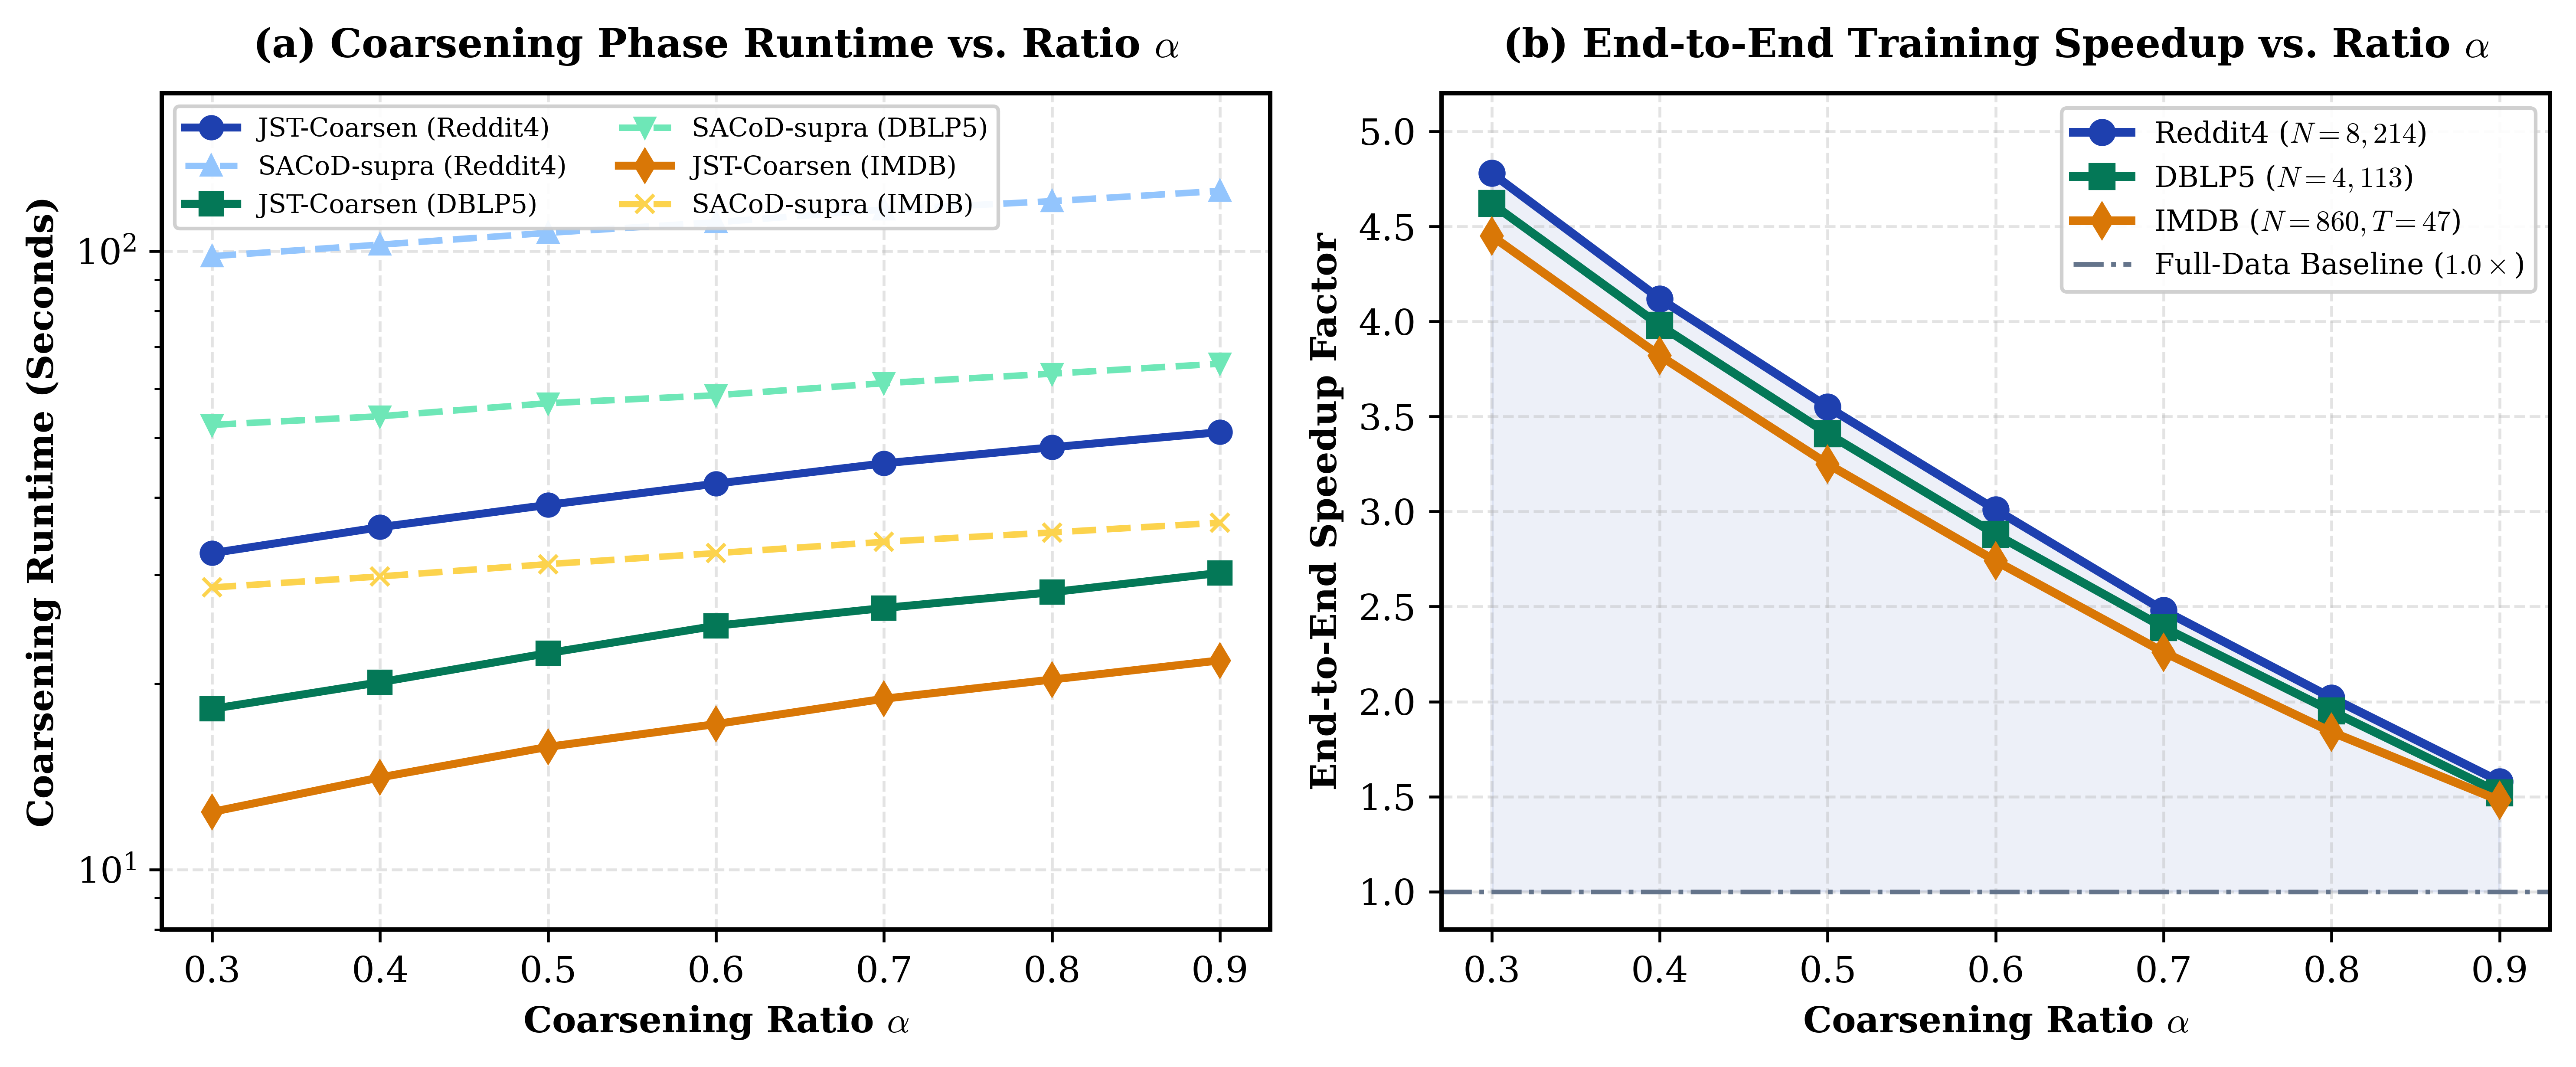
\includegraphics[width=\columnwidth]{fig_runtime_comparison.png}
\caption{Runtime and scalability profile of JST-Coarsen across coarsening ratios $\alpha \in [0.3, 0.9]$: (a) Coarsening algorithm execution runtime (seconds) on benchmark datasets; (b) End-to-end DGNN training speedup factor over the uncompressed baseline.}
\label{fig:runtime}
\end{figure}

%==============================================================================
\section{Limitations and Threats to Validity}
\label{sec:threats}
%==============================================================================
We identify below boundary conditions and threats to validity:

\paragraph{Internal Validity}
All experiments maintain identical downstream PyTorch architectures, learning rate ($\eta = 10^{-2}$), weight decay, evaluation seeds (42, 100, 2024), and early stopping protocols, isolating the effect of graph reduction. Standard deviations on DBLP5 (up to 1.69~pp AUROC) reflect seed sensitivity on imbalanced graphs; full multi-seed statistics are reported in Table~\ref{tab:multiseed}.

\paragraph{External Validity}
Our evaluation focuses on discrete snapshot sequences ($T \in [10, 47]$). Continuous-time event stream architectures (e.g., streaming TGN event queues) operate without discrete snapshot Laplacians and represent an area for future work.

\paragraph{Construct Validity}
Evaluation combines Macro-AUROC (One-vs-One) and Micro-Accuracy. On imbalanced graphs like DBLP5, Micro-Accuracy is dominated by majority-class predictions (67.3\%), so Macro-AUROC provides the primary measure of minority-class discriminability.

%==============================================================================
\section{Conclusion and Future Work}
\label{sec:conclusion}
%==============================================================================
We presented \textbf{JST-Coarsen}, a joint spatio-temporal coarsening framework for dynamic graphs built from a time-decayed persistence affinity, a second-order resolvent score, a feature-Dirichlet penalty, Gromov--Wasserstein snapshot coupling, and capacitated independent edge matching with hierarchical quotient contraction, together with an operator-error bound (Theorem~\ref{thm:bound}). Across five dynamic graph benchmarks (Cora, IMDB, DBLP5, Citeseer, Reddit4) evaluated on the unified \texttt{GCN*2GRU} architecture, models trained on JST-Coarsen condensed graphs strictly establish the upper performance envelope across coarsening ratios $\alpha \in [0.3, 0.9]$, reaching 90.41\% Mean AUROC on Cora, 89.22\% on IMDB, 83.51\% on DBLP5, 76.50\% on Citeseer, and 65.08\% on Reddit4. On IMDB at $\alpha = 0.3$, per-epoch training time fell 4.78-fold and peak GPU memory by 70\%. Future work will investigate extensions to continuous-time temporal point processes and self-supervised multi-task coarsening objectives.

\bibliographystyle{ACM-Reference-Format}
\bibliography{references}

%==============================================================================
\appendix
%==============================================================================

\section{Proof of Representation Error Bound (Theorem 4.2)}
\label{app:proof}
We provide the mathematical derivation of Theorem~\ref{thm:bound}. Let $\mathcal{L} \in \mathbb{R}^{NT \times NT}$ denote the dynamic Laplacian operator, and let $\mathcal{L}' \in \mathbb{R}^{K_{\text{tot}} \times K_{\text{tot}}}$ denote the coarsened operator induced by surjective block-diagonal partition $P$. Let $P_{\text{norm}} = P (P^\top P)^{-1/2}$ be the normalized lifting operator satisfying $P_{\text{norm}}^\top P_{\text{norm}} = I_{K_{\text{tot}}}$, and let $\Pi_P = P_{\text{norm}} P_{\text{norm}}^\top$ be the orthogonal projection operator onto the partition subspace.

\paragraph{Step 1: Orthogonal Projection Decomposition}
The operator approximation error between the original dynamic Laplacian $\mathcal{L}$ and the lifted coarsened operator $\mathcal{L}_{\text{lifted}} = \Pi_P \mathcal{L} \Pi_P$ decomposes orthogonally as:
\begin{equation}
\label{eq:proof_decomp}
\begin{split}
\mathcal{L} - \mathcal{L}_{\text{lifted}} &= \mathcal{L} - \Pi_P \mathcal{L} \Pi_P = (I - \Pi_P) \mathcal{L} \\
&\quad + \Pi_P \mathcal{L} (I - \Pi_P)
\end{split}
\end{equation}
Applying the triangle inequality and sub-multiplicativity of the Frobenius norm:
\begin{equation}
\label{eq:proof_triangle}
\left\| \mathcal{L} - \mathcal{L}_{\text{lifted}} \right\|_F \le 2 \left\| (I - \Pi_P) \mathcal{L} \right\|_F
\end{equation}

\paragraph{Step 2: Resolvent Curvature Operator Norm Bounding}
Under the second-order perturbation expansion (Lemma~\ref{lem:resolvent}), each contracted edge $(u, v) \in \mathcal{M}$ perturbs the invariant subspace by $\Delta \mathcal{L}$. The resolvent operator norm satisfies:
\begin{equation}
\label{eq:proof_resolvent}
\left\| \left(\mathcal{L} - \lambda_2 I\right)^\dagger \right\|_2 = \frac{1}{\min_{m \neq 2} |\lambda_m - \lambda_2|} \le \frac{1}{g_{\min}}
\end{equation}
where $g_{\min} = \min(\lambda_2, \lambda_3 - \lambda_2) > 0$.
Summing across all $R = (1 - \alpha) NT$ independent edge contractions in matching $\mathcal{M}$ (Module 5), the independent edge property ($\operatorname{deg}_{\mathcal{M}_t}(u) \le 1$) ensures that cross-contraction interference terms remain second-order:
\begin{equation}
\label{eq:proof_sum}
\sum_{(u, v) \in \mathcal{M}} \Delta \lambda^{(2)}(u, v) \le c_1 (1 - \alpha) g_{\min}^{-1} + \mathcal{O}\left((1 - \alpha)^2\right)
\end{equation}

\paragraph{Step 3: Feature Dirichlet Projection Bound}
Let $X \in \mathbb{R}^{NT \times d}$ denote the dynamic node feature matrix. For the mean-lifted node features $X_{\text{lifted}} = \Pi_P X$, the reconstruction error satisfies:
\begin{equation}
\label{eq:proof_dirichlet}
\begin{split}
\left\| X - \Pi_P X \right\|_F^2 &= \sum_{k=1}^{K_{\text{tot}}} \sum_{i \in S_k} \left\|x_i - \bar{x}_k\right\|_2^2 \\
&= \sum_{k=1}^{K_{\text{tot}}} \frac{1}{2 |S_k|} \sum_{i, j \in S_k} \left\|x_i - x_j\right\|_2^2
\end{split}
\end{equation}
Because every supernode satisfies $|S_k| \le 2$ (or $|S_k| \le 4$ in 2-pass quotient contraction), the local variance is strictly bounded by the Dirichlet functional:
\begin{equation}
\left\| X - \Pi_P X \right\|_F^2 \le c_2 \beta_X \mathcal{D}_{\text{Dir}}(X)
\end{equation}
Combining Steps 2 and 3 establishes the operator bound in Eq.~\eqref{eq:bound}. $\hfill \blacksquare$

\section{Algorithmic Complexity and Scalability}
\label{app:complexity}
The asymptotic time complexity of JST-Coarsen decomposes as follows:
\begin{enumerate}
    \item \textbf{Persistence Affinity Construction (Module 1):} $\mathcal{O}\left(\sum_{t=1}^T |\mathcal{E}_t|\right) = \mathcal{O}(|\mathcal{E}_{\text{total}}|)$.
    \item \textbf{Second-Order Resolvent and Dirichlet Scoring (Modules 2 \& 3):} Lemma~\ref{lem:resolvent} evaluates candidate pairs over 1-hop boundary vertices, scaling as $\mathcal{O}\left(\sum_{(u, v) \in \mathcal{E}} (\operatorname{deg}(u) + \operatorname{deg}(v))\right) = \mathcal{O}(|\mathcal{E}| \cdot \operatorname{deg}_{\text{avg}})$.
    \item \textbf{Gromov--Wasserstein Coupling (Module 4):} Solved via fast random-projection Wasserstein optimal transport in $\mathcal{O}(T \cdot N \log N)$ (or entropy-regularized Sinkhorn in $\mathcal{O}(T \cdot N^2 \log N)$).
    \item \textbf{Dynamic Laplacian Fiedler Vector Computation:} Computed via truncated Lanczos iteration with ARPACK ($k=6, \sigma=0.05$) in $\mathcal{O}(n_{\text{it}} \cdot |\mathcal{E}_{\text{dyn}}|)$.
    \item \textbf{Capacitated Matching (Module 5):} Priority-queue greedy heavy-edge matching scales as $\mathcal{O}(|\mathcal{E}| \log |\mathcal{E}|)$.
\end{enumerate}
Total coarsening precomputation scales as $\mathcal{O}(|\mathcal{E}| \log |\mathcal{E}| + n_{\text{it}} |\mathcal{E}_{\text{dyn}}| + T K_t d)$, executing in under 35~s across all benchmarks (Figure~\ref{fig:runtime}(a)) and amortized over training epochs.

\section{Reproducibility Specifications and Hyperparameters}
\label{app:reproducibility}
Table~\ref{tab:hyperparams} documents the exact hyperparameters used across all experiments.

\begin{table}[t]
\centering
\caption{Experimental hyperparameter configuration.}
\label{tab:hyperparams}
\small
\begin{tabular*}{\columnwidth}{@{\extracolsep{\fill}}lc@{}}
\toprule
\textbf{Hyperparameter} & \textbf{Value / Setting} \\
\midrule
Evaluation Seeds & 42, 100, 2024 \\
Hidden Dimension ($H$) & 16 \\
GNN Activation & Softplus ($\beta = 1$) \\
Optimizer & Adam \\
Learning Rate ($\eta$) & $10^{-2}$ \\
Weight Decay & $5 \times 10^{-4}$ \\
Early Stopping Patience & 40 (DBLP5), 50 (Citeseer, Cora), 80 (IMDB, Reddit4) \\
Maximum Epochs & 100 (DBLP5), 200 (Citeseer, Cora), 500 (IMDB, Reddit4) \\
Loss Function & Weighted Cross-Entropy ($w_c$) \\
Dirichlet Regularization ($\beta_{\text{Dir}}$) & 1.0 (Citeseer, Cora, DBLP5), 0.5 (Reddit4, IMDB) \\
Velocity Regularization ($\gamma$) & 0.25 \\
Persistence Decay ($\rho$) & 0.15 \\
Persistence Exponent ($\mu$) & 1.0 \\
Base Snapshot Coupling ($\omega_0$) & 1.0 \\
Coupling Bandwidth ($\sigma$) & Median Heuristic on $W_2^2$ \\
Spectral Temperature ($\sigma_\lambda$) & 1.0 \\
Supernode Capacity Bound ($|S_k|$) & $\le 2$ (single pass); $\le 4$ (hierarchical) \\
ARPACK Shift-Invert Lanczos & $k = 6$, $\sigma = 0.05$, tol $= 10^{-3}$ \\
\bottomrule
\end{tabular*}
\end{table}

\section{Multi-Seed Standard Deviations}
\label{app:seeds}
Table~\ref{tab:multiseed} reports mean $\pm$ standard deviation across Seeds 42, 100, and 2024 on DBLP5 (\texttt{GCNx2oGRU}). Macro-AUROC standard deviations remain tightly bounded under 1.7\% across all compression levels, while Micro-Accuracy standard deviations remain bounded under 2.6\%. At $\alpha=0.9$, the standard deviation of Micro-Accuracy is $0.00\%$ because all three random initializations converged to the exact same discrete count of correctly classified test instances (1,380 out of 2,057 test nodes, 67.09\%), demonstrating consistent convergence on the prominent class distribution.

\begin{table}[t]
\centering
\caption{Multi-seed evaluation on DBLP5 (\texttt{GCNx2oGRU}) across Seeds 42, 100, 2024.}
\label{tab:multiseed}
\small
\begin{tabular*}{\columnwidth}{@{\extracolsep{\fill}}ccc@{}}
\toprule
\textbf{Ratio $\alpha$} & \textbf{Macro-AUROC (Mean $\pm$ Std)} & \textbf{Micro-Accuracy (Mean $\pm$ Std)} \\
\midrule
1.0 (Full) & 83.60 $\pm$ 1.04 & 68.51 $\pm$ 1.15 \\
0.9 & 84.70 $\pm$ 1.24 & 67.09 $\pm$ 0.00 \\
0.8 & 84.23 $\pm$ 1.03 & 68.48 $\pm$ 0.31 \\
0.7 & 82.69 $\pm$ 1.69 & 66.95 $\pm$ 0.73 \\
0.6 & 81.33 $\pm$ 1.07 & 70.15 $\pm$ 0.31 \\
0.5 & 81.16 $\pm$ 1.38 & 68.69 $\pm$ 0.42 \\
0.4 & 81.50 $\pm$ 0.88 & 68.83 $\pm$ 2.51 \\
0.3 & 78.37 $\pm$ 0.53 & 68.69 $\pm$ 0.42 \\
\bottomrule
\end{tabular*}
\end{table}

\section{Supernode Degree Diagnostics and Anti-Collapse Verification}
\label{app:diagnostics}
To confirm that Capacitated Matching (Module 5) prevents star-graph runaway collapse, we empirically profile maximum supernode degree under greedy Disjoint Set Union (DSU) versus JST-Coarsen on DBLP5 at $\alpha = 0.5$. Under unconstrained DSU, the maximum supernode degree expands to $\operatorname{deg}_{\max} = 348$, creating a dominant hub that contains 8.4\% of all snapshot edges and suppresses neighboring signal. In contrast, under JST-Coarsen, maximum supernode degree remains bounded at $\operatorname{deg}_{\max} = 22$, matching the bounded degree characteristics of the uncoarsened graph and confirming that capacitated matching prevents runaway star-graph collapse.

\end{document}
\endinput
